\documentclass[10pt,journal]{IEEEtran}

\usepackage{amssymb}

\usepackage{tikz}
\usetikzlibrary{positioning,arrows,backgrounds,fit,matrix}
\usepackage{amsfonts}
\usepackage{amsmath}
%\usepackage[boxed,figure]{algorithm2e}
\usepackage[all]{xy}
\usepackage{paralist}
\usepackage{multirow}

% enumerate MOA* algorithm overview.
%\usepackage{enumitem}
%%

\newcommand\fBold[1]{\textbf #1\relax}

%error gave "unknown graphics extension: eps" in Bil Software machine
\usepackage{epstopdf}

% thesis document classes extended from iat paper
\usepackage{amssymb}

\usepackage[noend]{algpseudocode}
%\usepackage{setspace}
\makeatletter
\renewcommand{\ALG@beginalgorithmic}{\small}
\makeatother

%\usepackage{algorithmic}
\usepackage{algorithm}
\usepackage{colortbl}
\usepackage{color}

\usepackage{graphicx}
\graphicspath{{./figures/}}
\DeclareGraphicsExtensions{.eps}

\usepackage{comment}
% end of iat paper package extensions

\usepackage{tabularx}
\usepackage[footnotesize]{subfigure}

\newenvironment{definition}[1][Definition]{\begin{trivlist}
\item[\hskip \labelsep {\bfseries #1}]}{\end{trivlist}}

\begin{document}

\title{MOD* Lite}

\author{TO, FP}

\maketitle

\begin{abstract}
Path planning is a crucial issue for virtual environments where autonomous agents try to navigate from a specific location to a desired one. There are several algorithms developed for path planning, but several domain requirements make engineering of these algorithms difficult. In complex environments, considering single objective for searching and finding optimal or sub-optimal paths becomes insufficient. Thus, multi objective cases are distinguished and more complicated algorithms to be employed is required. It can be seen that more realistic and robust results can be obtained with these algorithms because they expand solution perspective into more than one criteria. Today, they are used in various games and simulation applications.

On the other hand, most of these algorithms are off-line  and delimitate interactive behaviours and dynamics of real world into a stationary virtuality. This situation reduces the solution quality and boundaries. Hence, the necessity of solutions where multi objectivity is considered in a dynamic environment is obvious. With this motivation, in this work, a novel multi objective incremental algorithm, MOD* Lite, is proposed. It is  based on a known complete incremental search algorithm, D* Lite. Solution quality and execution time requirements of MOD* Lite are compared with existing complete multi objective off-line search algorithm, MOA*, and better results are obtained.
\end{abstract}

% INTRODUCTION
\chapter{Introduction}
\label{chapter:introduction}

The problem of finding a path for an autonomous agent from an initial location to a destination location is a popular problem in real-world applications including robotics, virtual simulations or computer games and has been studied for many years. Thus, many solutions are proposed in computer science society for this issue. Proposed path planning algorithms can be classified into four categories: off-line algorithms \cite{Dijkstra:1959} \cite{AStarHart:1968}, on-line algorithms \cite{RTAStarKorf:1990}, incremental algorithms \cite{DStar:1994}, \cite{Koenig:2002}, \cite{FocussedDStarStentz:1995} and soft computing algorithms \cite{Tarapata:2007}, \cite{Pangilinan}. Off-line path planning algorithms try to find the whole solution before starting the execution, whereas on-line search algorithms require the planning and execution phases to be coupled, such that the agent repeatedly plans and executes the next movement. In dynamic or partially known environments, off-line path planning algorithms suffer from execution time, whereas on-line algorithms yield low quality solutions in terms of path length. Incremental heuristic search algorithms try to merge advantages of both approaches to obtain better execution time without sacrificing optimality. They reuse the information gained from previous iterations and improve it instead of calculating from scratch like off-line search methods. Soft computing algorithms generally come up with evolutionary solutions. Their main perspective is to evaluate and evolve solution quality by time. 

Existing incremental algorithms for path planning problem attempt to minimize path length. However, in many real-world problem domains we see that there are several objectives to be optimized concerning the solution (path) quality. Consider the navigation of an unmanned vehicle from one coordinate to another on a 3D terrain in a warfare setting. The navigation task is defined to be finding a path which is shortest but also the safest among all possibilities considering the existence of opponent forces in a partially known environment due to limited sensor capabilities. Note that shortest path may not be the safest one, on the contrary it might be the most dangerous one. And also the safest path may be the longest one which is unacceptable due to fuel consumption or time thresholds. 

There is a need to generalize the notion of quality of a path to meet specific requirements of complex application domains where several objectives (criteria) that cannot be transformed to each other exist. For example, in our unmanned vehicle example, it is not possible to transform the distance metric to the safety metric, and vice versa. This requirement raises the problem of handling decision making of multiple criteria at the same time. In this study; an incremental path finding algorithm called Multi-Objective D* Lite (MOD* Lite) which extends an existing incremental algorithm, Dynamic A* Lite (D* Lite) \cite{Koenig:2002}, is introduced. MOD* Lite \cite{Oral:2012} can be used in the design of an autonomous mobile agent facing with the problem of navigation in a partially known environment that needs to optimize a predefined set of independent objectives (criteria). The agent might have limited sensor capability and hence partially observe the environment, and furthermore need to optimize multiple objectives at the same time.

In order to show that MOD* Lite generates the optimal and sub-optimal solutions, also a new multi objective genetic path planning (MOGPP) algorithm is designed. This algorithm finds initial paths randomly and its population (solutions) evolve according to a fitness function. MOD* Lite is both compared against MOGPP and MOA* algorithm \cite{MOAStewart:1991}, an offline algorithm, on some test environments that are fully observable. The performance of MOD* Lite is also tested on several partially observable environments guaranteeing the optimal solutions but outperforming the MOA* and MOGPP versions modified for unknown environments.

The following chapters in this thesis are organized as follows: Chapter 2 gives the background and related work for this study. As MOA* is used in experimental studies and D* Lite is used as a base of proposed solution, these algorithms are also detailed in this chapter. The problem definition, characteristics of the environment and proposed solutions (MOD* Lite and MOGPP) are presented in Chapter 3. Experimental studies and their results are stated in Chapter 4. Finally, the conclusion and future studies are provided in Chapter 5.


% RELATED WORK
\chapter{Related Work}
\label{chapter:relatedwork}

The GRN control problem is a popular problem that has gained more attention with the advancements in
molecular biology in the last decade. The idea of intervening with the genes became possible with the
research on TFs and other dynamics in the protein biosynthesis. From the biological point of view, simple
pathways of genes were formulated for explaining certain phenomena in the~cell.

Lately, the research community has focused more on generic and complex interactions between genes, and GRNs
became an important tool; intervention problems have been formulated using GRNs~\cite{Datta03,Pal08,Pal06}.
Different mathematical frameworks and approaches have been used for devising mechanisms of intervention with
genes in order to accomplish some non-trivial goals. There are numerous useful examples of this intervention
mechanisms. For instance, targeted therapy is a cancer treatment technique based on suppressing the
expression of some genes in order to prevent cancerous behavior in cells~\cite{Green04}. Employing
mathematical models and computational techniques in undertaking the intervention problem would increase our
ability to devise more complex intervention~mechanisms.

Modeling the GRN control problem using PBNs is an approach widely used by the research
community~\cite{Kauffman93}. PBN model network dynamics and different approaches can be used for solving
control problems defined on this representation. Expressing the problem in terms of an MDP and using general
purpose MDP solving algorithms is an approach well suited to PBN representation. Examples of methods that use
Markovian and MDP concepts are the work of Shmulevich et al.~\cite{Shmulevich02} and the work of Datta et
al.~\cite{Datta03} who studied the dynamics of PBN model in the probabilistic context of Markov chains. The
work of Pal et al.~\cite{Pal05} explores an alternative model, namely context-sensitive probabilistic Boolean
network for the intervention~problem.

Our research group has already contributed to the control and intervention of GRN by developing novel
approaches based on PBN formulation of the network and different formulations of the intervention problem,
including MDP formulation~\cite{Abul04,Abul06,Tan08,Tan10,Tan10b}. The main focus on these previous works by
our group was formulating the GRN in PBN model and trying to solve the MDP problem in different settings and
exploring different aspects such as finite or infinite horizon reward mechanisms, factored representations of
the MDP problems, and improved modeling and solution techniques for plain and factored MDP problems.
Although our techniques have been effective and well received by the research
community~\cite{Abul04,Abul06,Tan08,Tan10,Tan10b}, we realized the need for incorporating partial
observability in the problem definition; and accordingly, the target of our approach described in this paper
is to develop appropriate solutions for the problem augmented to be partially~observable.

The need to cover partial observability has been realized by some other researchers; however, the problem has
not yet received enough and comprehensive attention. Datta et al.~\cite{Datta03} developed a finite horizon
control algorithms for GRNs; their algorithms can work with imperfect information. They modeled the gene
regulatory network as a PBN and used Markovian probabilities for their control algorithm, which is basically
an optimization algorithm based on dynamic programming. Bryce et al.~\cite{Bryce07} were first to model the
GRN control problem as a POMDP. Their approach makes use of PBN representation of the problem and their POMDP
formulation is similar to the PBN formulation. Their focus was on solving finite horizon problems, and
obviously they did not use a POMDP solver for solving the derived POMDP problem. They applied a probabilistic
planning algorithm for extracting an intervention mechanism for a finite horizon. Our approach described in
this paper is a major contribution to the literature because to the best of our knowledge it is the first
effort to develop a method that properly and comprehensively incorporates partial observability in handling
the control~of~GRNs.


% Proposed Solutions
\chapter{Proposed Solutions}
\label{chapter:proposedAlgorithm}

\section{Motivation}
% Definition of the problem 
Assume that an unmanned aerial vehicle (UAV) is taking off from an initial location. Its goal is trying to shoot an enemy unit on a predefined target location in an unknown dynamic environment. However, this enemy unit is protected by air defence units scattered on the terrain having different capabilities (hit ratios) and coverage areas. Each defence unit scans the space within its coverage areas to detect any threat. Due to its limited sensor capability, a UAV can only partially observe the environment. The air defence zones produce computable risk values for UAVs when they enter UAV's perceived sensor range. On the other hand; UAV has limited fuel and time, so it must locate and shoot the target quickly but the risk of being hit by an air defence unit must be minimized. This means that the UAV should find both shortest and safest path \textit{as quickly as possible}.

In this real-world problem, the UAV has to execute a planner and quickly find available paths. Also it must re-plan executed path when an unknown part of the environment become known or known parts are changed (i.e. a visible defence unit's coverage area changes, shrinks or enlarges; or defence unit is disabled / enabled) as it navigates. Mostly, evolutionary search algorithms focus on this issue and come up with several solutions like \cite{Peng_Xu_Zhang:2011}, \cite{Foo_Knutzon:2009}. However, It is obvious that these algorithms are insufficient for reflecting and adapting the dynamics of the environment as they are not incremental. One alternative could be to adapt off-line MOA* to unknown environments but it is grossly inefficient as it has to be restarted from scratch every time when some unknown part of the environment becomes known or known part changes.

Considering these issues within path planning perspective, a necessity of a solution can be observed clearly. Thus, a multi objective incremental path planning algorithm is designed and developed based on non-optimized version of D* lite \cite{Koenig:2002} in this study. This algorithm is called multi objective D* lite, or MOD* Lite \cite{Oral:2012}. To prove effectiveness of MOD* Lite,  an alternative solution based on a genetic algorithm, multi objective genetic path planner, or MOGPP is also developed. Both solutions, MOD* Lite and MOGPP are detailed in next sections.

\section{Multi Objective D*  Lite : MOD* Lite}
\subsection{Overview}
Multi-objective problems focus on considering more than one objective concurrently (at the same time). Consequently, \textit{all} scalar values and atomic operations (like addition, checking for equality, etc.) are to be converted into vectors of scalars. This causes all functions (cost, heuristic, etc.) to have $n$ dimensions if there are $n$ non-interacting objectives to be optimized. For two scalars a and b, there are three outcomes: $a<b$, $a>b$ or $a=b$. However; for two vectors $u$ and $v$, besides $u<v$, $u>v$ and $u=v$ there is a fourth alternative meaning that $u$ and $v$ cannot be compared. $u$ and $v$ are said to be \textit{equal} if all corresponding objective values are equal, or in other words;
\[ \forall n \in N;	 u_{n} = v_{n} \] where $N$ is total number of objective values for $u$ and $v$, $n$ is the $n^{th}$ objective value. For equality, both $u$ and $v$ must have the same cardinality, in other words, the same amount of objectives.

It could be said that $u$ \textit{dominates} $v$ if $u$ is better in at least one objective compared to $v$ or in other words, there is no objective of $v$ where it is better than any objective of $u$. Moreover, $u$ and $v$ are said to be \textit{non-dominated} if for at least one objective,  $u$ is better but for at least some other objective, $v$ is better. For instance, assume that we have two objectives to be minimized and let $\upsilon_{1}=[3,4], \upsilon_{2}=[4,6], \upsilon_{3}=[6,2] $. Here $\upsilon_{1}$ dominates $\upsilon_{2}$ but $\upsilon_{1}$ and $\upsilon_{3}$ are non-dominated.

MOD* Lite enables a user to define a set of objectives, $O_1, O_2, \cdots, O_n$ to be used in the evaluation of the quality of the candidate paths explored by an incremental algorithm. In that respect MOD* Lite is a domain-independent path search algorithm that can be used in any search problem where the environment is partially or fully observable. Note that for each objective $O_i$, the user needs to define whether $O_i$ is to be minimized or maximized. Each objective is assumed \textit{not to be transferable} to and \textit{non-interacting} with each other. This situation might reduce the number of objectives and should be considered out of this study, with a different algorithm. For the sake of simplicity, the execution and tests of MOD* Lite is restricted to the UAV domain example which has been introduced above with two objectives to be minimized, namely the distance and the degree of risk of danger.

\subsection{Environmental Properties}
\label{envProperties}
MOD* Lite applied to the UAV path finding task is illustrated in a 2-D grid based environment. It is easier to present the algorithm and also demonstrate its effectiveness on such a simple environment.

The environment is considered to be partially observable because of limited sensor capability of the agent. The agent can perceive the environment around her within a square region centered at the agent location. The size of the square is $(2v + 1)$ x $(2v + 1)$, where $v$ is the vision range. As the agent navigates, the known part of the environment gradually increases and it is presumed that agent is designed as having enough memory space to maintain all the perceived environment. It is assumed that the target is stationary and its location is known by the UAV agent at the initial step. Furthermore, the environment has randomly placed obstacles that cannot be traversed by the agent. The agent occupies only one grid cell. There are also threat zones in the environment. Threat zones produce predefined risk values which could effect the agent to fail reaching to the target cell. Threat zones are constructed up to three sub-zones. The innermost one is more hazardous than outer ones. So, if the agent has to enter a threat zone, it prefers to pass through outer levels. With threat zones, the agent must think about both the shortest and the safest path. The environment has randomly placed different sized threat zones.

\begin{figure}
\centering
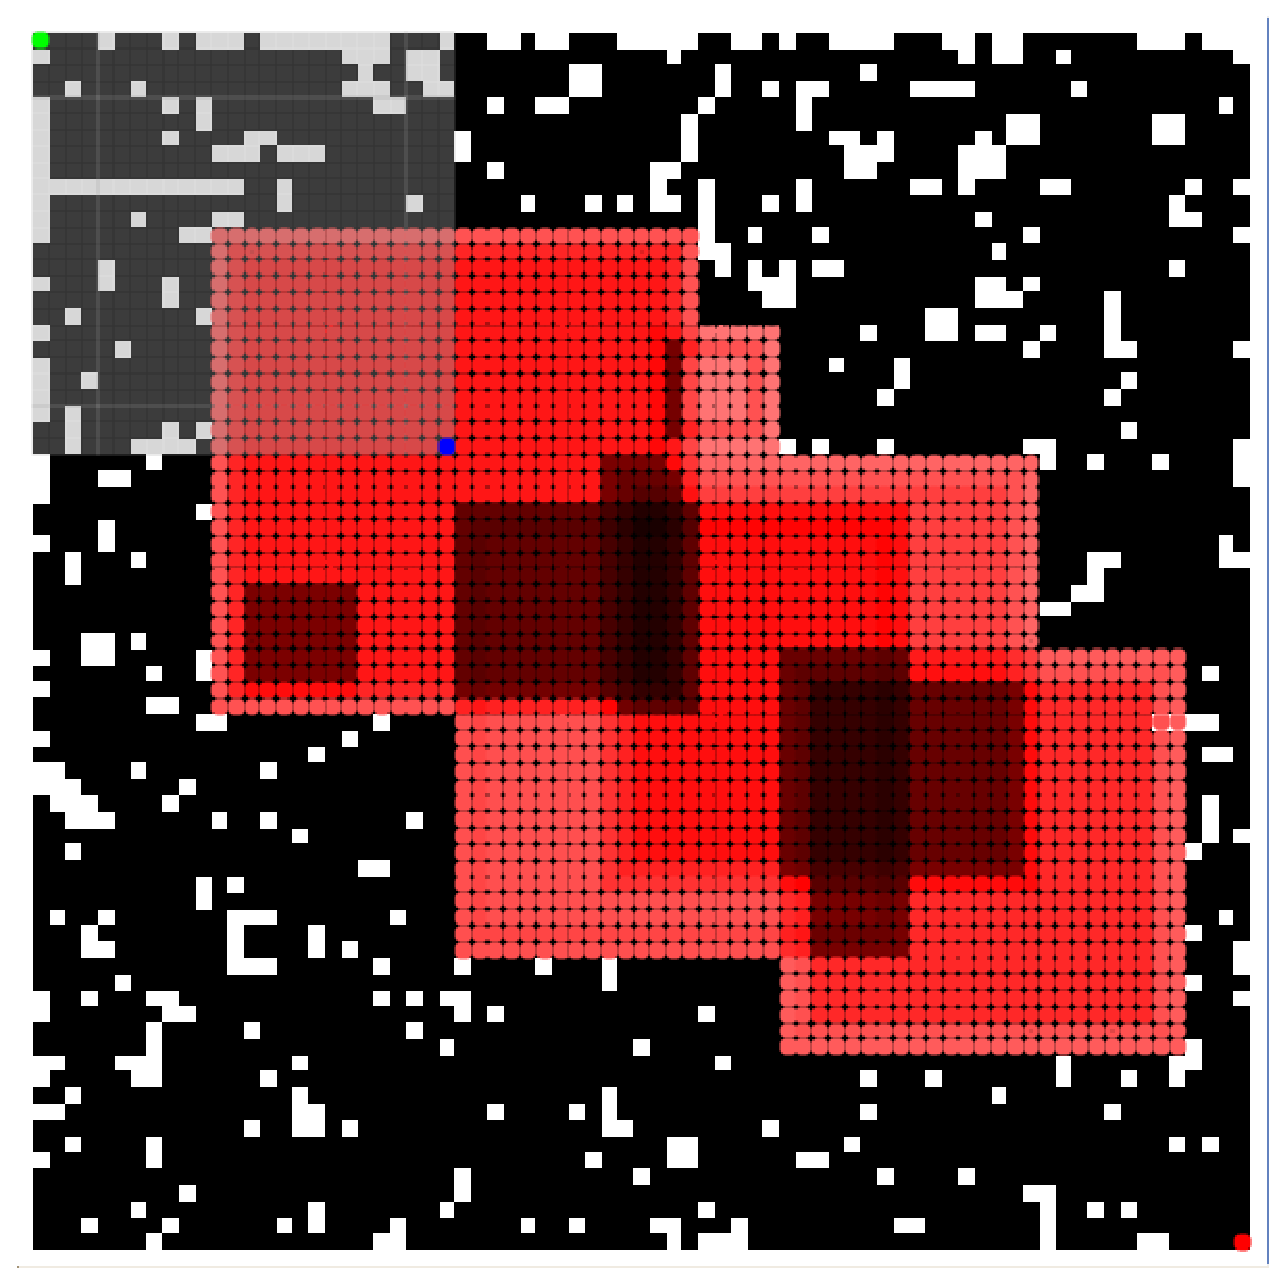
\includegraphics[width=4in]{modstarlite/75x75envPropertiesExample}
\caption{A 75 x 75 Visualized Grid Environment}
\label{fig:75x75envExample}
\end{figure}

A simple representation of 2-D grid environment is given in Figure \ref{fig:75x75envExample}. In this figure, white cells are obstacles and black cells are available ones. Agent can traverse all cells except for white ones. The UAV agent is initially placed on upper leftmost cell and painted as green. The target locates on the bottom rightmost and marked as dark red color. The lighter-red square areas represent threat zones. As two threat zones overlaps, the overlapped area becomes darker to represent that risk is increased exponentially on this area. The fogged gray area around UAV agent represents agent's vision range. As agent moves, this area is updated. Thus, agent always chooses the best available cell within her vision range with respect to actual target. This temporary target is marked with blue.

\subsection{The Components and Variables}
MOD* Lite is the multi-objective extension of D* Lite. It can be applied to any unknown dynamic multi-objective search problem where costs can change by time. Considering formal definition; $S$ denotes the set of states in search problem. $s_{start} \in S$ and $s_{goal} \in S$ are the initial and final (target) states, respectively. $pred(s) \subseteq S$ and $succ(s) \subseteq S$ can be used to find predecessors and successors of given state, $s$. The heuristic function $h(s, s')$ which estimates costs between $s$ and $s'$, cost function $c(s, s')$ which represents the actual cost traversing from $s$ to $s'$, actual cost function $g(s)$ and the $rhs(s)$, one-step-lookahead values of $g(s)$ functions are all inherited from D* Lite. However, as we have to consider more than one objective, these functions are to return vector values of scalars instead of scalars. Thus, $rhs(s)$ satisfies the condition

\[ rhs(s) = \left\{ \begin{array}{cc}
ObjectiveVector.MIN & \mbox{if $s=s_{start}$};\\
nonDom_{s' \in pred(s)}(sum(g(s'), c(s', s))) & \mbox{otherwise}.\end{array} \right. \] 

where ObjectiveVector.MIN stands for a vector with $n$ minimum values for an $n$ dimensional problem. These values could be $0$ or $\infty$ for minimization or maximization of objective, respectively. $sum()$ function implements vector summation and $nonDom()$ function returns the set of best non-dominated vectors corresponding to predecessors of any state $s$. Note that $nonDom()$ constructs a list of objective vectors, $rhs(s)$ and $g(s)$ function values are represented as a \textit{lists of objective vectors} where each objective vector in this list is non-dominated with others. An objective vector is a structure that holds values for each objective defined by problem (minimization or maximization). In case of having more than one objective, it is possible that there are more than one paths to a particular state that do not dominate each other. That's why each state might be represented by several vectors. In case we need to compare if one state is better than another, two sets of their vectors need to be compared as formulated below.

\begin{definition}
It can be said that $u$ \textit{completely dominates} $v$ iff $\forall x\in u$ and $\forall y\in v$; $x$ dominates $y$.
\end{definition}

Assume that $\upsilon_{1}=\{[2,5],[3,4]\}, \upsilon_{2}=\{[6,1],[5,2]\}, \upsilon_{3}=\{[3,5]\}$ are lists of objective vectors for three states. $\upsilon_{1}$ and $\upsilon_{2}$ are non-dominated whereas $\upsilon_{1}$ completely dominates $\upsilon_{3}$. 

It could be frankly said that the terms "greater than", "smaller than" and "equals" for scalar value comparison are replaced by "completely dominates", "completely dominated by" and "multi-objectively equals" for vectors of scalars. Non-domination is introduced and handled as the fourth case.

D* Lite introduces local consistency and inconsistency concepts with respect to comparing $g(s)$ and $rhs(s)$. A state is called {\it locally consistent} when $g(s)$ and $rhs(s)$ are equal, and {\it locally inconsistent} otherwise. A locally inconsistent state is referred as locally underconsistent if $g(s)<rhs(s)$ or locally overconsistent if $g(s)>rhs(s)$. In the case of non-domination of these functions, we introduce the concept of {\it local non-consistency}:

\begin{definition}
A state is referred as \textit{locally non-consistent} if its $g(s)$ and $rhs(s)$ values are non-dominated to each other. This inconsistency condition causes the state to reside on more than one solution because it can be understood that two or more predecessors of $s$ are non-dominated to each other.
\end{definition}

Other multi-objective operations are introduced in following subsections. The overall flow of MOD* Lite is given in Algorithm \ref{algMain}.

%% The main algorithm.
\begin{algorithm}
	\caption{Main loop of MOD* Lite}
	\label{algMain}
	%\begin{spacing}{0.5}
	{\fontsize{9}{9}\selectfont
    \begin{algorithmic}[1] % line numbering every line
      \Function{calculateKey}{s}
      	\State $k_{2}$(s)= nonDom(g(s), rhs(s))
      	\State $k_{1}$(s) = sum(h($s_{start}$, s), $k_{m}$, $k_{2}$(s))
      	\State \Return $[k_{1}(s), k_{2}(s)]$
      \EndFunction
   	  \Statex
      \Function{initialize()}{}
      	\State $U = \varnothing $
      	\State $k_{m}$ = ObjectiveVector.MIN
      	\ForAll{$s \in S$}
     		\State rhs(s)=g(s)=ObjectiveVector.MAX
     	\EndFor
      	\State rhs($s_{goal}$) = ObjectiveVector.MIN
      	\State U.insert($s_{goal}$, calculateKey($s_{goal}$))
	  \EndFunction
	  \Statex
	  \Function{plan()}{}
      	\State initialize()
      	\State computeMOPaths()
      	\While{$true$}
    	      	\State solutionPaths = generateMOPaths()
    	      	\If{solutionPaths = null} there is no known path \EndIf
    	      	\State Wait for any weight cost to change;
    	      	\If{Any weight cost changes}
    	      		\State $k_{m}$ = sum($k_{m}$, h($s_{goal}$, $s_{start}$))
    	      		\ForAll {Changed weight costs of edges(u,v)}
    	      			\State Update cost c(u,v)
    	      			\State updateVertex(u)
    	      		\EndFor
		      	\State computeMOPaths()
    	      	\EndIf
		\EndWhile
  	  \EndFunction
    \end{algorithmic}}
    %\end{spacing}
\end{algorithm}

Basically, D* Lite tries to make all states locally consistent. Locally inconsistent states are maintained in  a priority queue (U) with their key values and expanded considering priority values. However, locally non-consistent states cannot be maintained in such a queue due to the non-domination of their key values, which are also set of objective vectors. If two keys cannot be dominated by each other, they should be criticized in the same manner. Thus, a more convenient structure; a directed acyclic state expansion graph instead of a priority queue which uses topological ordering of states with respect to the key domination, is presented. In this model, the graph (U) contains set of nodes each represented by a state and its key value. When a state is to be added into U with $insert(state, key)$ operation, key value is compared with all existing nodes' key values. If the new state dominates some state, an edge is introduced from the new state to this state. No edge connection is done in case of multi objectively equality and non-domination. As a result, incoming and outgoing degrees of a node $s$ correspond to the number of nodes that \textit{dominates} $s$ and the number of nodes that are \textit{dominated by} $s$, respectively. The node(s) with incoming degree 0 are the non-dominated nodes where none of other nodes could dominate. $topKey()$ and $topKeys()$ return the key value(s) of nodes with minimum incoming degree. $pop()$ returns and removes the state (all its incident -incoming and outgoing- edges are also removed from the graph) with minimum incoming degree. Another strategy for $pop()$ operation could be removing the state with maximum outgoing degrees where the number of outgoing degree of a state $s$ presents that how many states are dominated by $s$. Also, these two methods could be combined where two topologically ordered lists, one is for minimum incoming degrees and the other is for maximum outgoing degrees, are maintained and a state which has both minimum incoming and maximum outgoing degrees according to these lists could be selected. As these strategies could be set to applied domain according to its requirements, we choose selecting and removing from minimum incoming degrees list. If more than one nodes exist with minimum degree, one of them is selected randomly. $remove(state)$ operation removes a given state and its incident edges from graph. An example of a state expansion graph with states and their corresponding key values is given in Figure \ref{fig:graph1}. Incoming degrees of nodes are given as a list in the figure.

\begin{figure}
\centering
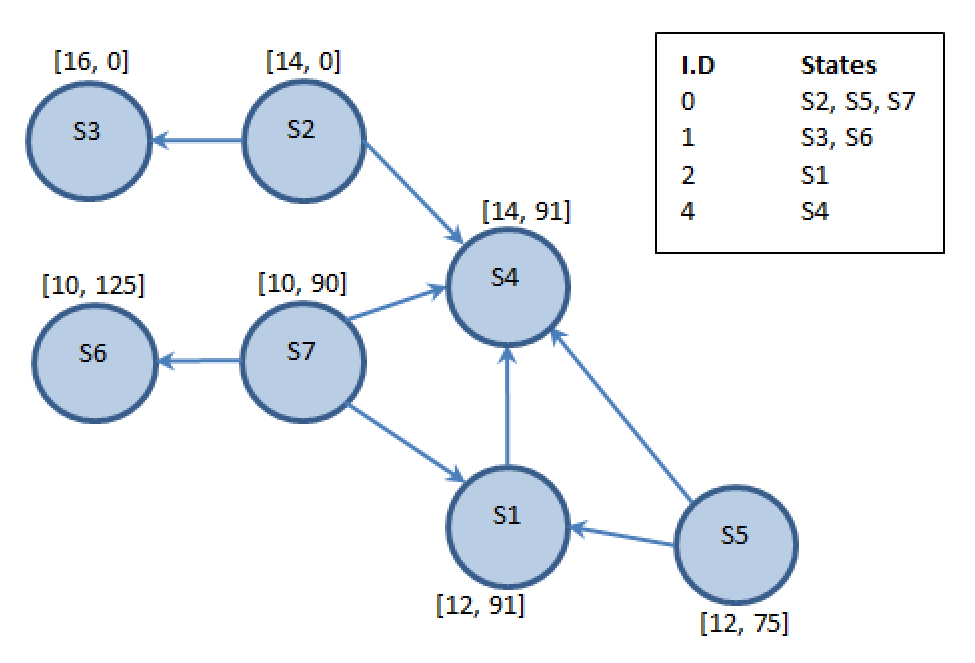
\includegraphics[width=4in]{modstarlite/graph1v2}
\caption{Directed Acyclic State Expansion Graph}
\label{fig:graph1}
\end{figure}

Addition of a new state to the state expansion graph is illustrated in Figure \ref{fig:graph2}.  $S8$ is  "the new" state to be added, the dashed directed edges are established between $S8-S1$, $S8-S4$ and $S8-S5$ because $S8$'s key can only dominate keys of nodes $S1, S4$ and $S5$. None of the existing states' keys can dominate $S8$, so incoming degree of $S8$ becomes 0. This addition also effects the incoming degrees list where the changed positions are highlighted in the figure. Addition of $S8$ increments the incoming degrees of $S1$, $S4$ and $S5$ by 1 so their positions are shifted down.

\begin{figure}
\centering
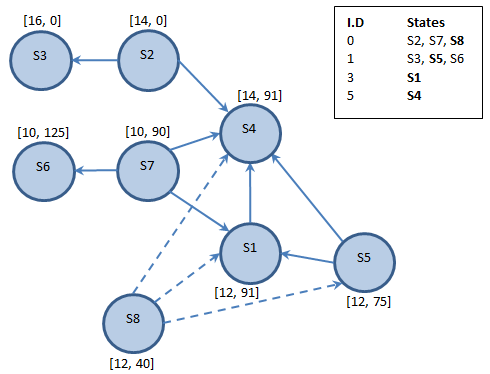
\includegraphics[width=4in]{modstarlite/graph2v2}
\caption{State Expansion Graph after Adding State $S8$}
\label{fig:graph2}
\end{figure}

\subsection{Key Formulation}
In the previous subsection, it is stated that the directed acyclic graph structure is used to determine expansion of nodes in state space with their \textit{keys}. The basic idea behind the calculation of keys is similar with D* Lite, with slight modifications. As MOD* Lite is considered in a multi-objective setting, key value is stated as a vector with two components: $k(s) = [k_{1}(s);k_{2}(s)]$ where these components are set of objective vectors. $k_{2}(s)$ is calculated by finding the \textit{non-dominated list} of $g(s)$ and $rhs(s)$, where $k_{2}(s)= nonDom(g(s), rhs(s))$. The other component, $k_{1}(s)$  is calculated as vector summation of $h(s_{start}, s), k_{m}$ and $k_{2}(s)$. Calculation of $k(s)$ can be seen in lines \{2 and 3\} in Algorithm \ref{algMain}. $k_{m}$ is used for heap reordering as defined in  D* Lite.

\begin{algorithm}
	\caption{Update Vertex \& Compute Multi-Objective Paths}
	\label{algUpdate}
    \begin{algorithmic}[1]
   	  \Function{updateVertex}{u}
   	  	\If{$u \neq s_{goal}$}
   	  		\State $rhs(u) = nonDom_{s' \in succ(u)}(sum(c(u,s'), g(s')))$
   	  	\EndIf
   	  	\If{$u \in U$} U.remove(u) \EndIf
   	  	\If{!equals(g(u), rhs(u))}
   	  		\State U.insert(u, calculateKey(u))
   	  	\EndIf
   	  \EndFunction
    	  \Statex
      \Function{computeMOPaths()}{}
		\While{dominatesAll(calculateKey($s_{start}$), U.topKeys())}
		% OR !equals(rhs(s_{start}, g(s_{start}))$}
			\State $k_{old}$ = U.topKey()
	      	\State u = U.pop()
	      	\State $k_{new}$ = calculateKey(u)
	      	\If{$k_{old}$.completelyDominates($k_{new}$) }
	      		\State U.insert(u, $k_{new}$)
	      	\ElsIf{rhs(u).completelyDominates(g(u))}
	      		\State g(u) = rhs(u)
	      		\ForAll{$s \in pred(u)$} $updateVertex(s)$ \EndFor
	      	\ElsIf{g(u).completelyDominates(rhs(u))}
	      		\State g(u) = ObjectiveVector.MAX
	      		\ForAll{$s \in pred(u) \cup \{u\}$} $updateVertex(s)$ \EndFor
	      	\Else
	      		\State g(u) = nonDom(g(u), rhs(u))
	      		\ForAll{$s \in pred(u)$} $updateVertex(s)$ \EndFor
	      	\EndIf
		\EndWhile
	  \EndFunction
	\end{algorithmic}
\end{algorithm}

\subsection{Details of MOD* Lite}
MOD* Lite is based on  D* Lite algorithm as introduced in the previous section. There are fundamental differences due to the structures used and the way the solution paths are maintained. The pseudocode of MOD* Lite is given in Algorithms \ref{algMain}, \ref{algUpdate} and \ref{algPathGen}.

First of all, searching order of MOD* Lite is from goal to start state, like D* Lite. The main function of MOD* Lite first calls $initialize()$ to set up the execution in Algorithm \ref{algMain}. This function calculates the key value for goal state, adds it into U and sets the rhs value to a \textit{MIN} objective vector, which has minimized n values for n-objectives. These values can be $0$ for minimized-objective and $\infty$ for maximized-objective. Then, proper $g(s)$ values are calculated considering all objectives with $computeMOPaths()$. Finally, paths are generated with these $g(s)$ values. If a weight cost is changed in the environment, corresponding states are re-expanded and only related weights are updated. Notice that this cost change might happen for only one objective or several objectives at the same time.

The $computeMOPaths()$ pseudocode is given in Algorithm \ref{algUpdate} line \{7\}. The termination criteria of this function is where the key of $s_{start}$ dominates all the top keys returned from U. Until it terminates, the top state is sequentially selected from top states of U and expanded. While expanding a state, the domination between g and rhs values of corresponding state is observed. If $rhs(s)$ values completely dominate $g(s)$ values, local underconsistency case occurs. We apply the same strategy with D* Lite, update g value with rhs and update weights for all predecessors of s with $updateVertex()$. If $g(s)$ values completely dominate $rhs(s)$ values, the case is locally overconsistency. Simply g value for this state is set as \textit{MAX} objective vector, which is $\infty$ for minimized-objective and $0$ for maximized one, and current state weight is updated with its predecessors' weight. The third case occurs when g and rhs values can not completely dominate each other, \textit{locally non-consistency}. In this case, g value is updated with non-dominated values of g and rhs values and again predecessors of current state is updated. Keeping non-dominated values of g and rhs enables to keep track of each non-dominated successors' information.

To update a weight of a state, MOD* Lite uses $updateVertex(u)$ shown in Algorithm \ref{algUpdate} line \{1-6\}. It simply adds corresponding state to or removes from U according to given criteria. While updating $rhs(u)$ except goal state, non-dominated objective values of multi-objectively summed $c(u,s')$ and $g(s')$ are established and used.

After state expansion operation is finalized and corresponding $g(s)$ values are set, multi-objective paths are generated via these $g(s)$ values by given pseudocode in Algorithm \ref{algPathGen}. Path generation is achieved in two phases: setting parent(s) for each non-dominated successor of expanding state and constructing paths by following (backtracking) these parents. The first phase is performed from the start to the goal state whereas the second is from the goal to the start state. 

A queue is used to keep track of expanding states which is shown in line \{2\}. This queue initially has $s_{start}$ only. Thus, starting from $s_{start}$, the while loop iterates until this queue becomes empty. Finding a goal state is not considered as a termination criteria because other non-dominant paths might be available. As expanding a state, we refer to set \textit{it} as a parent to its successors indicated between lines \{7-36\}.

Before expansion of a state $s$, non-dominated successors are found first with respect to multi-objective summation of $c(s,s')$ and $g(s')$ as shown in line \{5\}. If a successor $s'$ is found in non-dominated successors list, it has a potential to have $s$ as a parent. For each non-dominated successor $s'$, first parents list of $s$ is checked. If $s$ does not have any parent, which only occurs iff $s=s_{start}$, for sure $s'$ does not have any parent as well. In this case, $s$ is added  as a parent of $s'$ with corresponding cost $c(s,s')$. Parents of a state are kept in a map where keys of this map are parents and values are cumulative costs which is consumed to reach that state from start through corresponding parent. These costs are used to determine elimination of existing parents when a new one is considered to be added. This idea will be elaborated later.

% Indentations are used make visualization better.
\begin{algorithm}
	\caption{Path Generator Algorithm}
	\label{algPathGen}
    \begin{algorithmic}[1]
    		\Function{generateMOPaths()}{}
			\State expandingStates.add($s_{start}$)
    			\While{!expandingStates.isEmpty()}
    				\State s = expandingStates.poll()
				\State nonDomSuccs = $nonDom_{s' \in succ(s)}$(sum(c(s, s'), g(s'))
    				\ForAll{$s'\in nonDomSuccs$}
    					\If{s.parents() = null}
    						\State s'.parents().put(s, c(s, s'))
    					\Else
    						\State cumulativeC = sum(c(s, s'), s.parents().values())
    						\If{s'.parents() = null}
    							\State s'.parents().put(s, cumulativeC)
    						\Else
							\ForAll {$s'' \in s'.parents()$}
								\If{equals(s'.parents(s''), cumulativeC) OR completelyDominates( s'.parents(s''), cumulativeC)}
									\State \textbf{break}
								\ElsIf{completelyDominates(cumulativeC, s'.parents(s''))}
									\State s'.parents().remove(s'')
									\State s'.parents().put(s, cumulativeC)
								\Else
									\ForAll{$cC \in cumulativeC$}
										\ForAll{$eC \in s'.parents(s'')$}
											\If{eC.equals(cC) OR eC.dominates(cC)}
												\State cumulativeC.remove(cC) 
												\State \textbf{break}
											\ElsIf{cC.dominates(eC)}
												\State s'.parents(s'').remove(eC) 
												\State \textbf{break}
											\EndIf
										\EndFor
										\If{s'.parents(s'') = null}
											\State s'.parents().remove(s'')
										\EndIf
									\EndFor
									\If{!cumulativeC = null}
											\State s'.parents().put(s, cumulativeC)
									\EndIf
								\EndIf
							\EndFor    						
    						\EndIf
    					\EndIf
    					\If {s'.parents.contains(s) AND !expandingStates.contains(s')}
    						\State expandingStates.add(s')
    					\EndIf
    				\EndFor
    			\EndWhile
    			\State solutionPaths = construct paths recursively traversing parents
    			\State \Return solutionPaths
    		\EndFunction
	\end{algorithmic}
\end{algorithm}

If $s$ has predefined parents (starting from \{9\}), a cumulative total cost is calculated for $s'$ in line \{10\}. This cost is multi-objective summation of $c(s, s')$ and aggregated cost values of parents of $s$. Notice that the algorithm proves that parents' costs of a state are always non-dominated to each other, so the aggregated cost values contain \textit{all} parents' \textit{all} costs. These cost values express all non-dominated solution costs to reach that state. If $s'$ does not have any parent up to now (\{11\}), $s$ is added as a parent of $s'$ with cumulative cost. Else, each existing parent of $s'$, say $s''$ should be compared with the cumulative cost. These operations are shown in lines between \{13-32\}. Here, if $s''$ has same cost with or better cost (determined by completely domination term) than cumulative cost, needless to say that $s$ is not required to be added as a parent to $s'$. Otherwise, if cumulative cost completely dominates $s''$, it can be inferred that one can reach $s'$ from $s$ in a better way than $s''$. Thus, $s''$ is removed from parents of $s'$ and $s$ is added with the cumulative cost. The fourth possibility occurs when costs of $s''$ and cumulative costs do not completely dominate each other. In this situation, each cost in cumulative costs is compared with each cost of $s''$ costs. Equality or domination probabilities causes to remove corresponding cost from its list. At the end of the comparison, $s''$ is removed from parents of $s'$ if all of its costs are dominated (lines \{29-30\}) and $s$ is added as a parent if cumulative costs still have non-dominated cost (lines \{31-32\}).

After organizing parents of $s'$, it is decided to expand it in following iterations. If $s$ is successfully added as a parent and expanding states queue does not already have it, $s'$ is added to the tail of the queue. This can be seen in lines \{33-34\}.

When all non-dominated parents are properly set from start to goal state, these parents can be followed recursively starting from goal towards start state and multi-objective paths are constructed. Finally, all found paths have non-dominated path costs regarding to each other.

\section{A Multi Objective Genetic Path Planner : MOGPP}

Many real-life optimization problems are NP-hard where optimal solutions could not be found in polynomial time. As evolutionary computing methods are classified as stochastic soft-computing methods and can be applied to NP-hard problems, several genetic algorithms are developed with respect to this problem \cite{Pangilinan}, \cite{Peng_Xu_Zhang:2011}. To show that MOD* Lite gives feasible and qualified solutions, it is a must to compare it with a stochastic evolutionary method. Thus, a multi objective genetic path planner, MOGPP is also developed in the scope of this study.

\subsection{Overview}

Multi objective genetic path planner (MOGPP) proposed in this study is an alternative solution for finding paths on virtual environments considering multiple objectives. It proposes a classical genetic algorithm structure with crossover and mutation operations where each individual represents a valid path from initial location to target. Experimental and performance results show that MOGPP finds paths in exponential times with respect to MOD* Lite, which are detailed in next section. The chromosome structure, fitness function, crossover, mutation and details of the MOGPP are given in following subsections.

\subsection{Chromosome Representation}

Like all evolutionary algorithms, MOGPP come up with a population where each individual of the population is represented by a chromosome structure. This structure simply stands for a valid path from initial location to target, a legal solution for the problem. Thus, each gene in chromosome is a \textit{cell} in this valid path. As the solution path' s lengths differ from each other, the chromosome lengths may diversify.

\subsection{Fitness Function}

The fitness function is crucial to evaluate a chromosome which is tested for suitability for the environment under some consideration. As the genetic algorithm proceeds, it is expected that the fitness value of the "best" chromosome increases as well as the total fitness of the population as a whole.

The fitness function used in MOGPP is given as follows; \[F(i) = [\dfrac{1}{pathLength(i)^{2}}], [\dfrac{1}{exposuredRisk(i)^{2}}] \] which is the fitness function of individual $i$ in population. This function is represented by a vector of objectives, where first objective is inverse of path length square of corresponding individual and second objective is inverse of calculated exposured risk square during this path. The purpose of fitness function is to yield better results when an individual's path is shorter and safer. On the evaluation process, these fitness values of all individuals in the population are added multi objectively and evaluation value is calculated. The evolution of population is determined by this total fitness value.

\subsection{Crossover Operation}

In genetic algorithms, crossover operation is used to vary the chromosomes and generate new individuals from existing ones. But, to breed new individuals and to use the operators borrowed from natural genetics, the parents should be selected first. There exists many selection operations for genetic algorithms. For MOGPP, roulette-wheel selection method is used to keep the algorithm simple. With this way, greater fitness evaluation owner chromosomes have bigger opportunity to be selected. This mechanism facilitates the population to evolve.

As a single chromosome stands for a valid path in MOGPP, new generated children should also obey this rule. Thus, genetic operations must guarantee that new generated children are consistent and have valid paths. For crossover operation used in MOGPP, assume that two parents' paths are represented by 
\begin{gather*}
P(i)=\lbrace \varsigma, ..., c_{i-1}, c_{i}, c_{i+1}, ..., \tau \rbrace \\
P(j)=\lbrace \varsigma, ..., c_{j-1}, c_{j}, c_{j+1}, ..., \tau \rbrace
\end{gather*}
for $i$ and $j$ individuals. $\varsigma$ and $\tau$ shows initial and target locations, respectively. While crossover, an intersected cell of these paths is determined. Then, each path is split up into two sub-paths referencing by this cell. If this cell is $c_{i} = c_{j}$, the splitting operation is done as follows
\begin{gather*}
P(i)_{1}=\lbrace \varsigma, ..., c_{i-1} \rbrace \\
P(i)_{2}=\lbrace c_{i}, c_{i+1}, ..., \tau \rbrace \\
P(j)_{1}=\lbrace \varsigma, ..., c_{j-1} \rbrace \\
P(j)_{2}=\lbrace c_{j}, c_{j+1}, ..., \tau \rbrace
\end{gather*}
The concatenation of swapped sub-paths generate new individuals
\begin{gather*}
P'(i)=\lbrace P(i)_{1}, P(j)_{2} \rbrace \\
P'(j)=\lbrace P(j)_{1}, P(i)_{2} \rbrace 
\end{gather*}
$P'(i)$ and $P'(j)$ are the new crossovered paths for parents $i$ and $j$. Also, visualized representation of crossover operation is given in Figure \ref{fig:xover}.

\begin{figure}
\centering
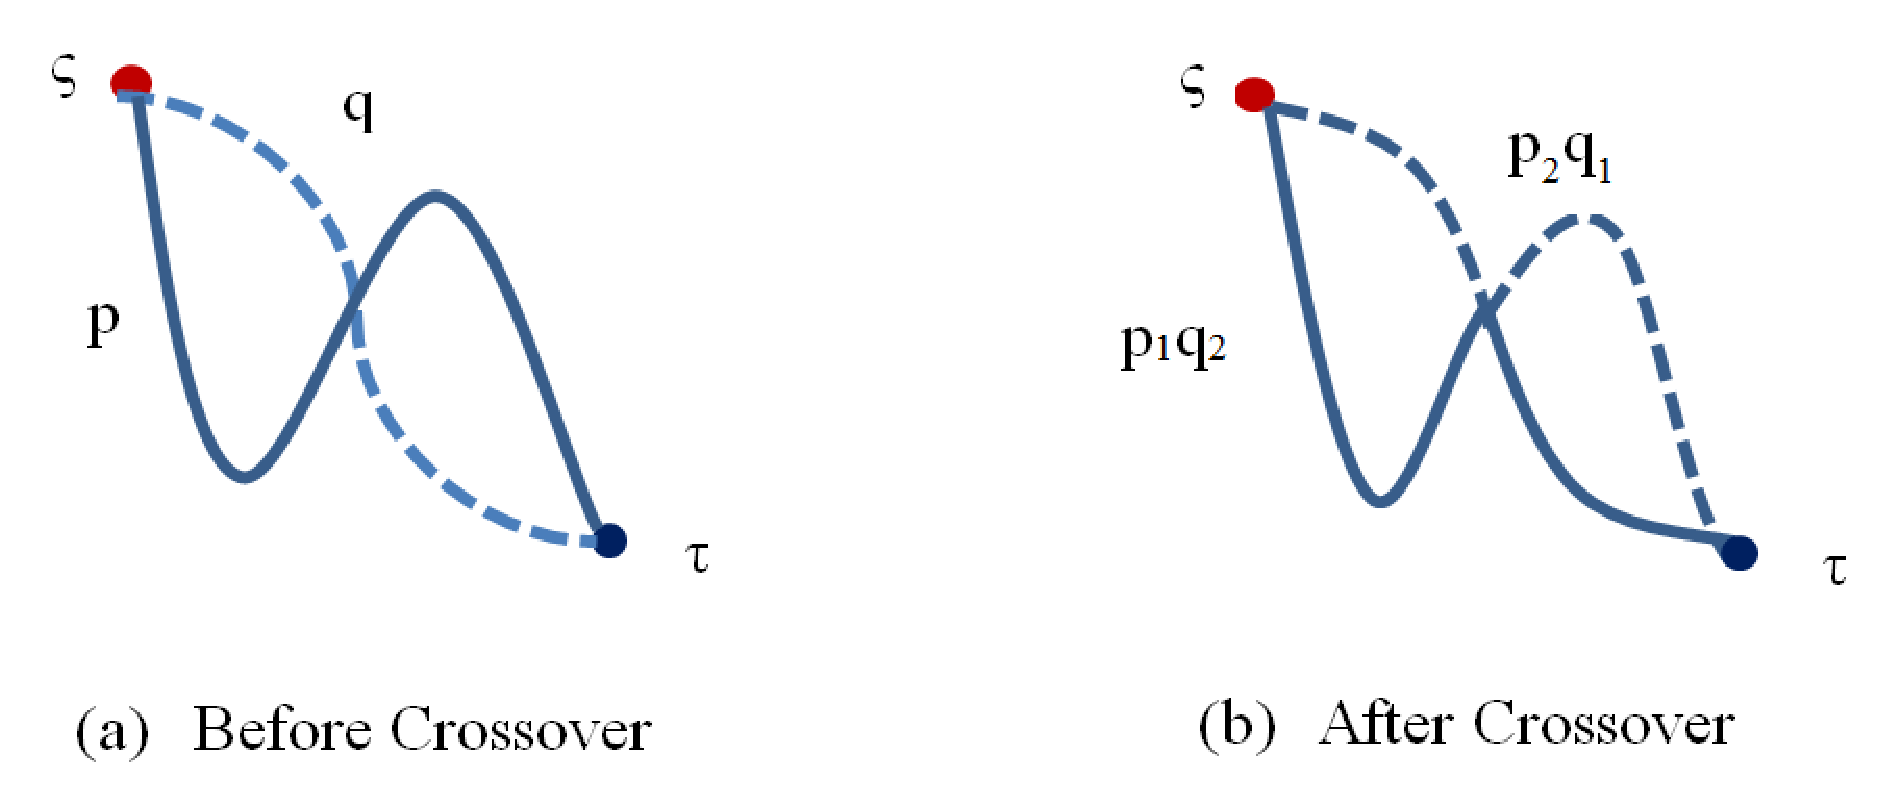
\includegraphics[width=4in]{mogpp/xover}
\caption{Crossover Operation}
\label{fig:xover}
\end{figure}

\subsection{Mutation Operation}

In genetic algorithms, mutation is used to maintain genetic diversity of the population. In MOGPP, with respect to given chromosome structure; a cell from corresponding individual' s path is selected randomly first. This cell is the reference point to split up the path into two sub-paths. Then, the sub-path which contains target location is thrown away and a random path to the target is generated instead. The visualization of mutation is given in Figure \ref{fig:mutation}.

\begin{figure}
\centering
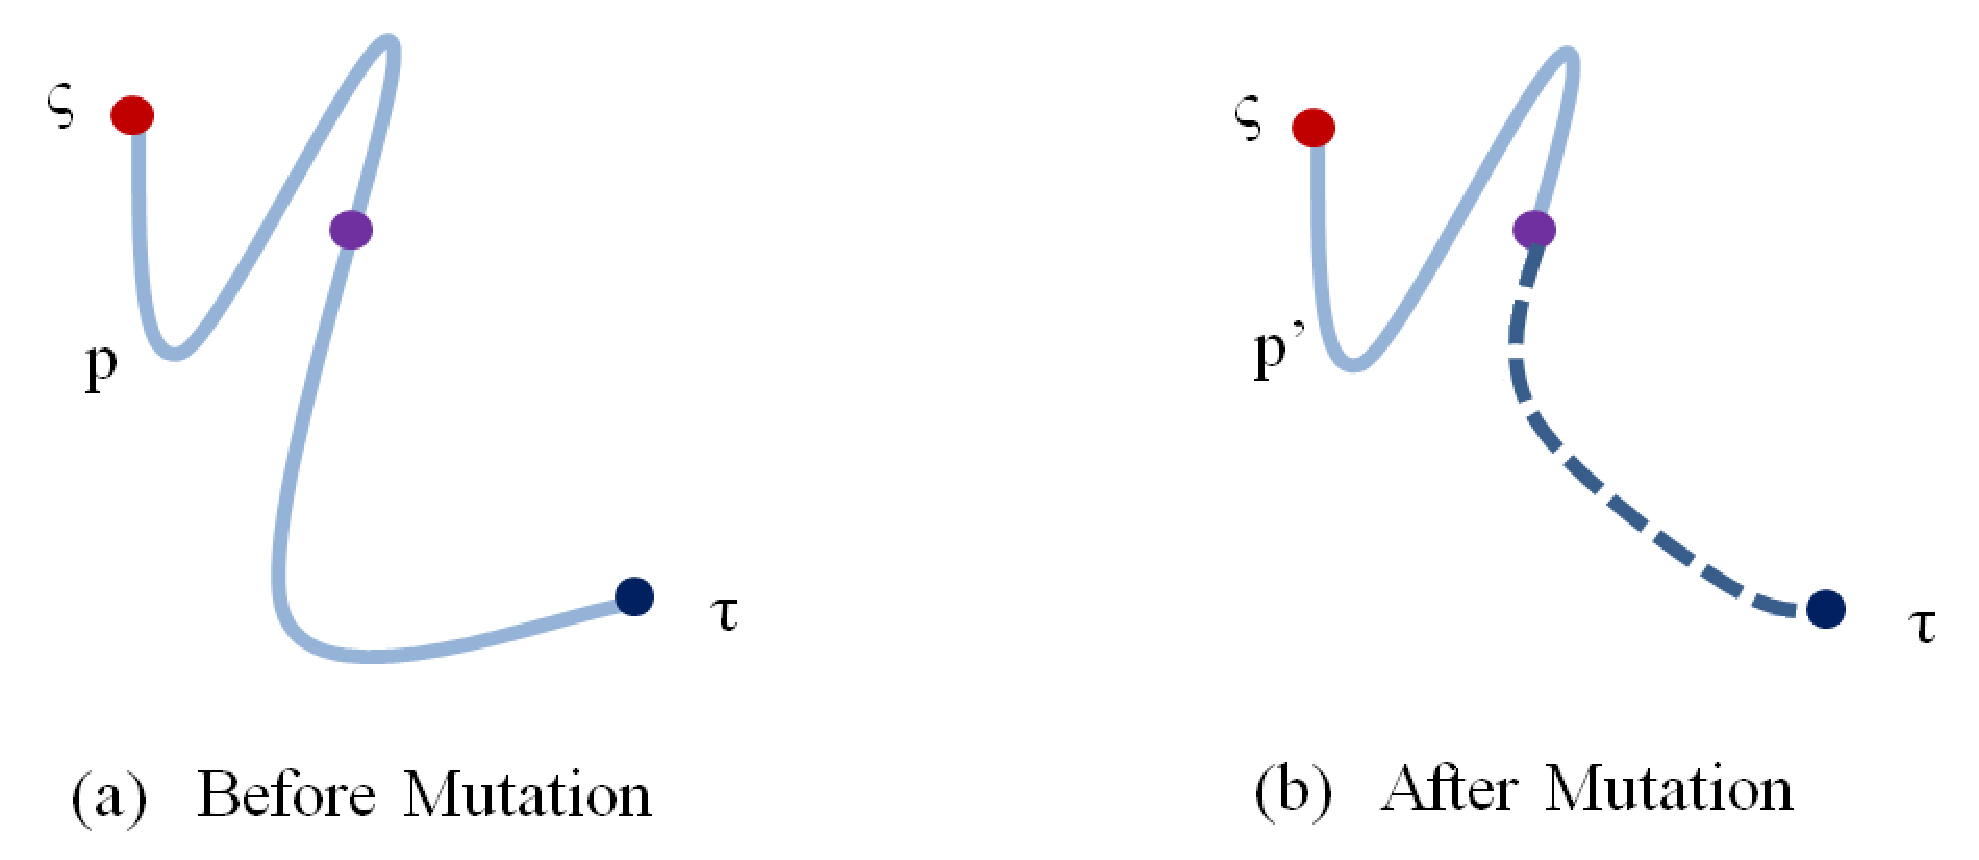
\includegraphics[width=4in]{mogpp/newMutation}
\caption{Mutation Operation}
\label{fig:mutation}
\end{figure}

\subsection{Details of Algorithm}

As mentioned above, MOGPP is designed based on a simple classic genetic algorithm structure. Main loop of MOGPP is given in Algorithm \ref{algMOGPP}.

\begin{algorithm}
	\caption{MOGPP : Main Loop}
	\label{algMOGPP}
    \begin{algorithmic}[1]
    	  \Function{evolve()}{P}
	  	\State $P' = \varnothing$
	  	\State $P'.addAll(elites(P))$
	  	\While{$P'.size < P.size$}
	  		\State $parents = selectParents(P)$
	  		\State $crossover(parents)$
	  		\State $mutate(parents)$
		  	\State $P'.addAll(parents)$
	  	\EndWhile
	  	\State \Return $P'$
      \EndFunction
   	  \Statex
      \Function{initializePopulation()}{}
      	\State $P = \varnothing$
      	\For{$i = 1 \to POPULATION\_SIZE$}
      		\State $P(i) = generateRandomPath(\varsigma, \tau)$
      	\EndFor
      	\State $evaluate(P)$
		\State \Return $P$
	  \EndFunction
	  \Statex
	  \Function{plan()}{}
      	\State $P = initializePopulation()$
      	\While{$reached\ to\ MAX\_ITERATION$}
    	      	\State $P = evolve(P)$
    	      	\State $evaluate(P)$
		\EndWhile
		\State \Return $bestIndividuals(P)$
  	  \EndFunction
	\end{algorithmic}
\end{algorithm}

Initialization of algorithm starts with $plan()$ function. At first, random valid paths from initial location ($\varsigma$) to the target ($\tau$) are generated. Notice that these paths do not contain any ties, to simplify and speed up genetic operators' processes.

Each generated path represents an individual in population. These individuals are kept in a directed acyclic graph to cope with multi objectivity. The vertices and edges represent individuals and domination of multi objective path costs of these individuals, respectively. If a path cost of an individual dominates to other's, an edge is established between these individuals' vertices. Non domination and equality do not come up with an edge. When an individual is generated and desired to be added to population, the cost function of this individual is compared with existing individuals' costs and required edge connections are established. The directed acyclic graph structure has the same essence and representation with MOD* Lite' s priority structure, which was detailed in previous section. 

After population initialization, all individuals are evaluated with respect to their fitness functions. The evaluation gives better results when an individual's path is shorter and safer. Total fitness value is calculated by adding all individuals' fitness values multi objectively. This value increases while population is evolving.

The evolution process is applied to all individuals of a population. When a population is evolving, predefined number of best individuals are transferred to new population first. Then, two individuals are selected as parents by roulette wheel selection method. This method gives higher chances to the individuals which have better fitness functions to be selected. After two parents are selected, crossover and mutation is applied with predefined distinct probabilities.

After a predefined number of iterations (the maximum iteration count), algorithm is halted and elite individuals are taken as multi objectively best results.

Notice that the amount of initially generated individuals - population size -, maximum iteration count of evolution, number of elite individuals selected on each evolution phase, crossover and mutation probabilities should be predefined and set before the execution of MOGPP.


\section{Experimental Results}
\label{chapter:experiments}

MOD* Lite is a domain independent algorithm and can be applied to any virtual environment with given $n$ objectives. These objectives could be whether \textit{maximized} or \textit{minimized}. The vital assumption about objectives is their independence from each other. If two objectives could effect each other in a positive or negative manner, this might reduce or expand objectives vector size, which is out of this work's scope. Thus, we assume that each defined objective is considered in different perspective and can not be transferred to each other.

The algorithm is tested on various environments with different scenarios. However, as it is not possible to exemplify all possible cases, specific and several extreme conditions are selected for experiments. MOD* Lite is compared with MOA* that guarantees optimal solutions in fully observable multi objective environments and MOGPP, a classic genetic solution which can be used for finding paths with multi objective cases.

For testing, all algorithms are implemented in Java language and run under Linux environment which has Intel(R) Core(TM) i7-2600 CPU @ 3.40GHz and 8 GB of RAM with -Xmx6192m parameter for JVM.

All tests are done on 2-D grid maps as detailed in Subsection \ref{envProperties}. In these tests, the agent tries to find available non-dominated best paths with respect to two objectives, path length and risk taken from threat zones. Thus, the agent endeavours to minimize both objectives and tries to find \textit{shortest} and \textit{safest} paths.

For all test cases, several parameters of MOGPP algorithm must be tuned. For instance; number of elitist individuals are $5$, population count and maximum iteration are $50$, and cross-over and mutation ratios are taken as $0.8$ and $0.05$, respectively. As MOGPP constructs initial paths randomly, each execution of the algorithm might not give exactly same results at the same execution time even the maps are equal. Thus, all given execution times and selected paths are considered as the average of 10 different executions for MOGPP.

\subsection{Fully Observable Tests}

First of all, it must be shown that MOD* Lite is complete and gives optimal and/or sub-optimal results in fully observable environments. The performance comparison is done in two dimensions, execution times and paths they generate (path quality), respectively.

In the first set of tests, randomly generated fully observable maps with different sizes (20 x 20, 40 x 40, 60 x 60, 80 x 80, 100 x 100, 120 x 120, 140 x 140 and 160 x 160), are used. Each of these maps have nearly 25\%-30\% percent threat zone and 14\%-16\% percent obstacle ratio. Agent's initial and target locations are taken as farmost cells on diagonal. For this case, execution times and generated paths' costs for different sized maps are given in Figure \ref{fig:rand_fully} and Table \ref{table:randPaths}. As seen from path qualities, MOA* finds optimal results and MOD* Lite finds optimal and/or sub-optimal results while gradually increases on the computation time manner. Although MOGPP works on similar times with MOD* Lite, it fails to find optimal or sub-optimal paths  especially for large scaled maps. One could set maximum iteration and population count to larger numbers to converge path quality to optimality, but this case increases execution time exponentially. Thus, more modest parameters are chosen for MOGPP to enforce the algorithm to yield reasonable results within expected time. 
 
Notice that taken risk values depend on environmental properties and should not be compared between different sized maps.

\begin{figure}
\centering
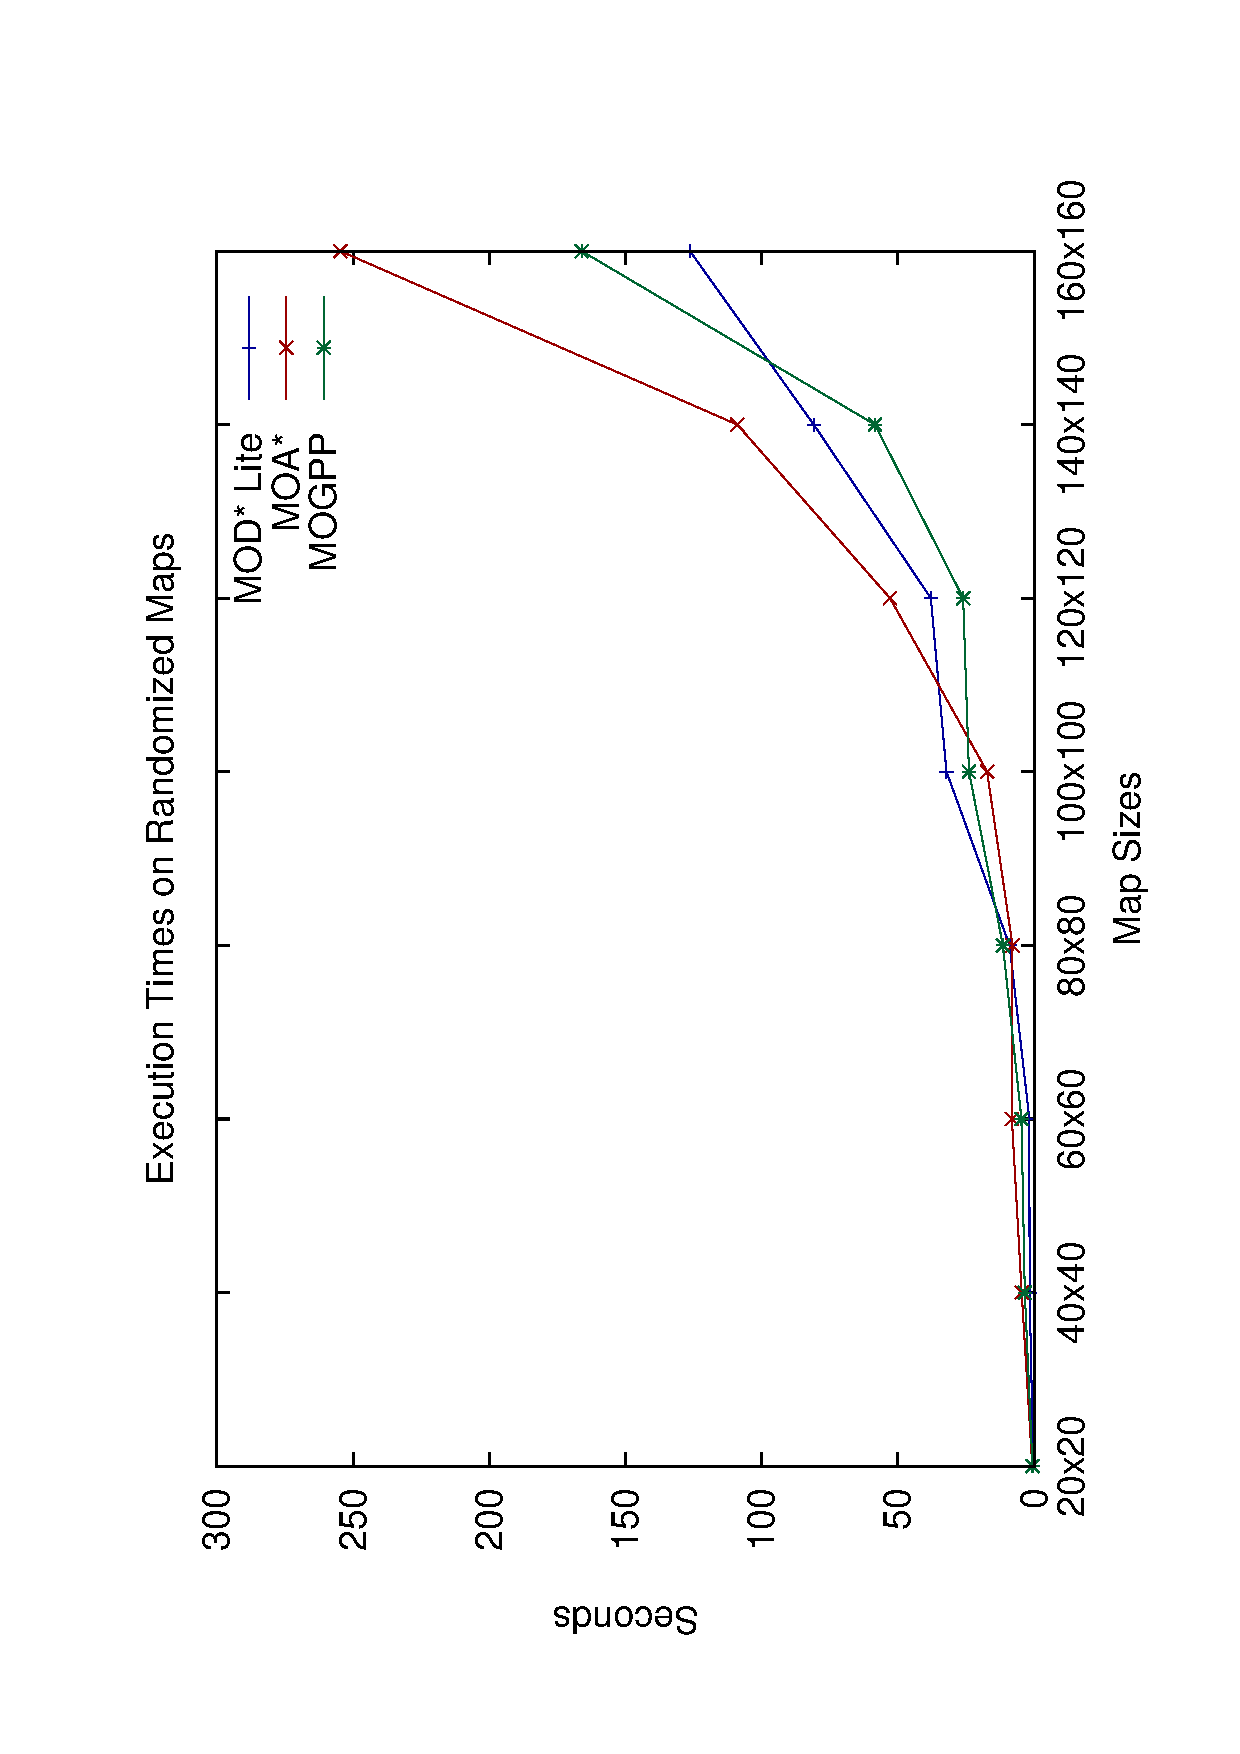
\includegraphics[width=2.5in, angle=270]{experimental/randomized_normal}
\caption{Execution Times of Randomly Generated Fully Observable Maps}
\label{fig:rand_fully}
\end{figure}

\begin{table}[ht]
	\caption{Non-dominated Path Costs For Randomized Maps}
	\centering
    \begin{tabular}{l l l l}
        \hline
        Map Size	&  MOD* Lite	&	MOA*		&	MOGPP \\ [0.5ex] \hline
        20 x 20		&	(39,90)		&	(39,90)		&	(41,916)
		   \cr		&	(43,0)		&	(43,0)		&	(43,408)\\
		   \\ 
        40 x 40		&	(79,9)		&	(79,9)		&	(89,2789)
		   \cr		&	(81,0)		&	(81,0)		&	(103,1239)
		   \cr		&				&				&	(105,296)\\
		   \\
		60 x 60		& 	(119,0)		&	(119,0)		&	(151,1970)
		   \cr		&				&				&	(169,549)
		   \cr		&			  	&				&	(181,426)\\
		   \\
        80 x 80		& 	(159,198)	&	(159,58)	&	(213,6382)
		   \cr		& 	(161,0)		&	(161,0)		&	(237,2007)
		   \cr		& 				&				& 	(263,1581)
		   \cr		& 				&				& 	(269,955)
		   \cr		& 				&				& 	(285,942)\\
		   \\
        100 x 100	&	(199,885)	&	(199,885)	&	(285,15804)	
		   \cr    	&	(201,708)	&	(201,708)	&	(295,14130)
		   \cr    	&	(203,0)		&	(203,0)		&	(299,14099)
		   \cr	  	& 				&				&	(305,10979)
		   \cr	  	& 				&				&	(341,9851)
		   \cr	  	& 				&				&	(377,177)\\		   
		   \\
        120 x 120	&	(239,0)		&	(238,0)		&	(371,12817)
		   \cr		&				&				&	(399,7346)\\
		   \\
        140 x 140	&	(279,45)	&	(279,45)	&	(445,10920)
		   \cr		&	(281,42)	&	(285,12)	&	(483,5281)        
    	   \cr		&				&	(303,0)		&	(515,4000)
 		   \cr		&				&			 	&	(517,3520)\\
 		   \\
        160 x 160	&	(319,0)		&	(319,0)		&	(545,7530)
		   \cr		& 			 	&			 	&	(547,4602)\\ [1ex]
        \hline
    \end{tabular}
	\label{table:randPaths}
\end{table}

In the second set of tests, each algorithm is executed on handcrafted maps with same sizes, threat zone and obstacle ratio with randomized tests as indicated in previous test case. These maps are also assumed fully observable and agent's initial and target locations are as farmost cells on diagonal. All handcrafted test environments \textit{guarantee} that at least two non-dominated paths will be available. Execution times are shown in Figure \ref{fig:hand_fully} and generated paths' costs are given in Table \ref{table:handPaths}.

\begin{figure}
\centering
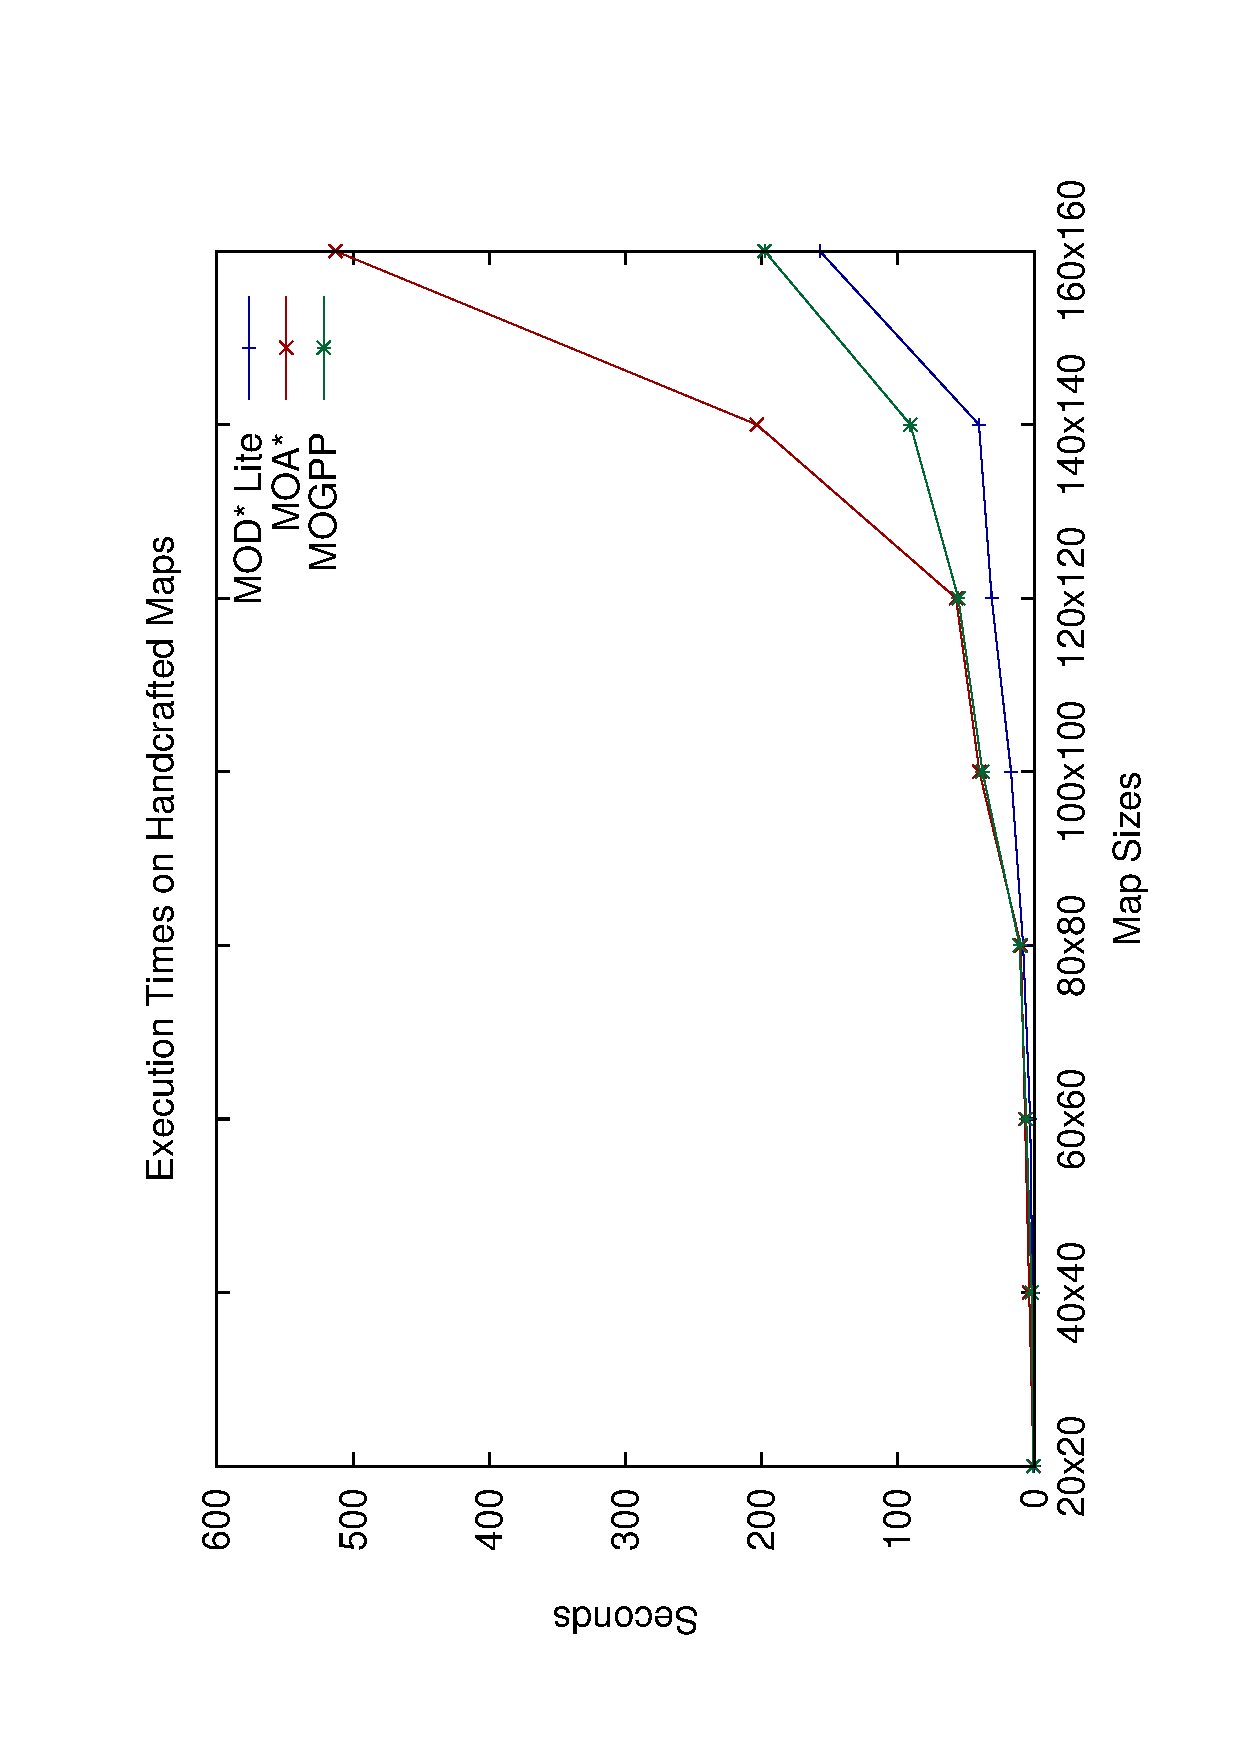
\includegraphics[width=2.5in, angle=270]{experimental/handcrafted_normal}
\caption{Execution Times of Handcrafted Fully Observable Maps}
\label{fig:hand_fully}
\end{figure}

\begin{table}[ht]
	\caption{Non-dominated Path Costs For Handcrafted Maps}
	\centering
    \begin{tabular}{l l l l}
        \hline
        Map Size  &  MOD* Lite  & 	 MOA*  		&  	MOGPP\\ [0.5ex] \hline
        20 x 20   &	(39,264)	&	(39,264)	&	(39,1614)
		   \cr    &	(41,258)	&	(43,6)		&	(41,394)
   		   \cr    &	(45,0)		&	(45,0)		&	(47,264)
   		   \cr	  &				&				&	(49,0)\\ 
   		   \\
        40 x 40   & (79,528)	&	(79,528)	&	(95,1637)
		   \cr	  &	(81,352)	&	(81,352)	&	(115,880)
		   \cr	  &	(91,156)	&	(91,156)	&  
		   \cr	  &	(97,0)		&	(97,0)		& \\
		   \\
        60 x 60   & (119,243)	&	(119,243)	&	(159,4761)
		   \cr	  & (123,33)	&	(123,33)	&	(165,1979)
   		   \cr	  & (127,0)		&	(127,0)		&	(167,165)
   		   \cr	  &				&				&	(233,99)\\ 
   		   \\
        80 x 80   & (159,129)	&	(159,129)	&	(223,2327)
		   \cr	  &	(161,69)	&	(161,69)	&	(291,1627)
		   \cr	  &	(163,0)		&	(163,0)		& \\
		   \\
        100 x 100 &	(199,30)	&	(199,30)	&	(311,4827)
		   \cr	  &	(201,6)		&	(201,6)		&	(327,3042)
		   \cr	  &	(203,0)		&	(203,0)		&	(341,1989)
   		   \cr	  &				&				&	(353,45)
   		   \cr	  &				&				&	(365,0)\\ 
   		   \\
        120 x 120 & (239,77)	&	(239,77)	&	(363,11340)
		   \cr	  & (241,44)	&	(241,44)	&	(413,8821)
		   \cr	  &			   	&	(261,0)		&	(417,4613)		   
		   \cr	  &			   	&				&	(455,3830)
		   \cr	  &			   	&				&	(517,1292)\\
		   \\
        140 x 140 & (210,1774)	&	(210,1774)	&	(306,16134)
           \cr	  & (212,1728)	&	(212,1344)	&	(336,10836)           
   		   \cr	  & (214,40)	&	(214,40)	&	(368,6510)
		   \cr	  &	(244,0)	   	&	(244,0)		&	(390,4876) 
		   \cr	  &			   	&				&	(500,3335)   
		   \cr	  &			   	&				&	(514,2328)\\
		   \\
        160 x 160 & (319,913)	&	(319,601)	&	(497,41016)
           \cr	  & (321,581)	&	(321,354)	&	(563,19675)
   		   \cr	  & (323,0)		&	(323,0)		&	(719,14811)
		   \cr	  &			   	&				&	(859,9448)\\ [1ex]
        \hline
    \end{tabular}
	\label{table:handPaths}
\end{table}

In execution times in Figure \ref{fig:hand_fully}, it can be seen that MOGPP increases gradually instead of an exponential growth especially on large scaled maps. However, its path quality is not good enough when compared to MOD* Lite and MOA*' s results.

There exists a remarkable point that MOA* has nearly similar results with MOD* Lite in path quality manner. This case shows that even MOD* Lite is based on partially observable dynamic environments, it could also give \textit{as good results as} MOA* on stationary and fully observable environments and can be applied on those environments.

\subsection{Partially Observable Tests}

As discussed in previous sections; the main difference of MOD* Lite from existing classic path planning or evolutionary based algorithms is its adaptivity to partially observable dynamic environments. To show this advantage, partially observable tests are done with randomized maps of sizes 60 x 60, 80 x 80, 100 x 100 and 120 x 120. On these maps, agent's initial and target locations are chosen to be the furthermost cells in the environment. For each map, agent' s sensor range was set between 10\% to 60\% and execution times were observed. An example search space of MOD* Lite with 30\% sensor range can be seen in Figure \ref{fig:initialSearch}. In this figure, agent is depicted with a cyan dot. The fogged gray area represents agent' s sensor range and drawn purple path through temporary goal (blue dot) can be seen.

\begin{figure}
\centering
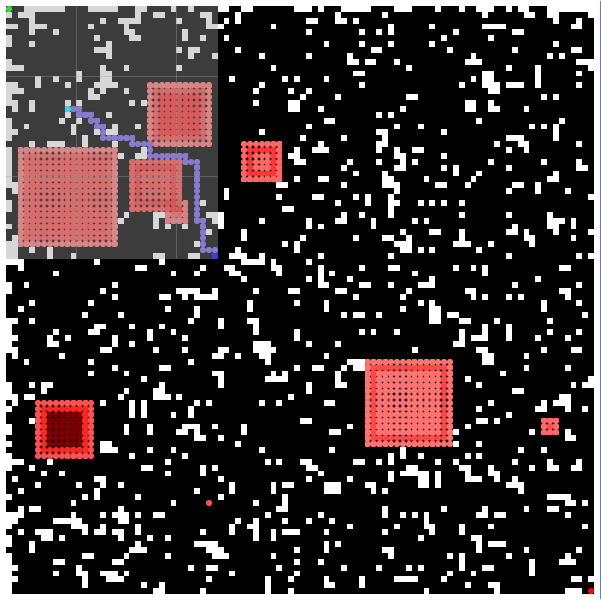
\includegraphics[width=2.5in, angle=270]{experimental/initialSearch}
\caption{A 100x100 Partially Observable Map with 30\% Sensor Range}
\label{fig:initialSearch}
\end{figure}

In these tests, the agent starts to plan a path towards the nearest available cell within its sensor range -the temporary goal- to the actual goal with respect to Manhattan Distance. After planning, consider that agent has found three paths with costs $(15, 200)$, $(18, 230)$ and $(23, 260)$. In such cases, the agent tends to choose the path with cost $(18, 230)$, the median of paths. This ad-hoc strategy could be set explicitly according to the domain that the algorithm works on. Afterwards, it starts to follow the chosen path. When new cells are available or a weight of a cell is changed within sensor range, agent reassigns the temporary goal and re-executes the path planner algorithm. This process iterates until the agent reaches to the desired goal location.

\begin{figure}
\centering
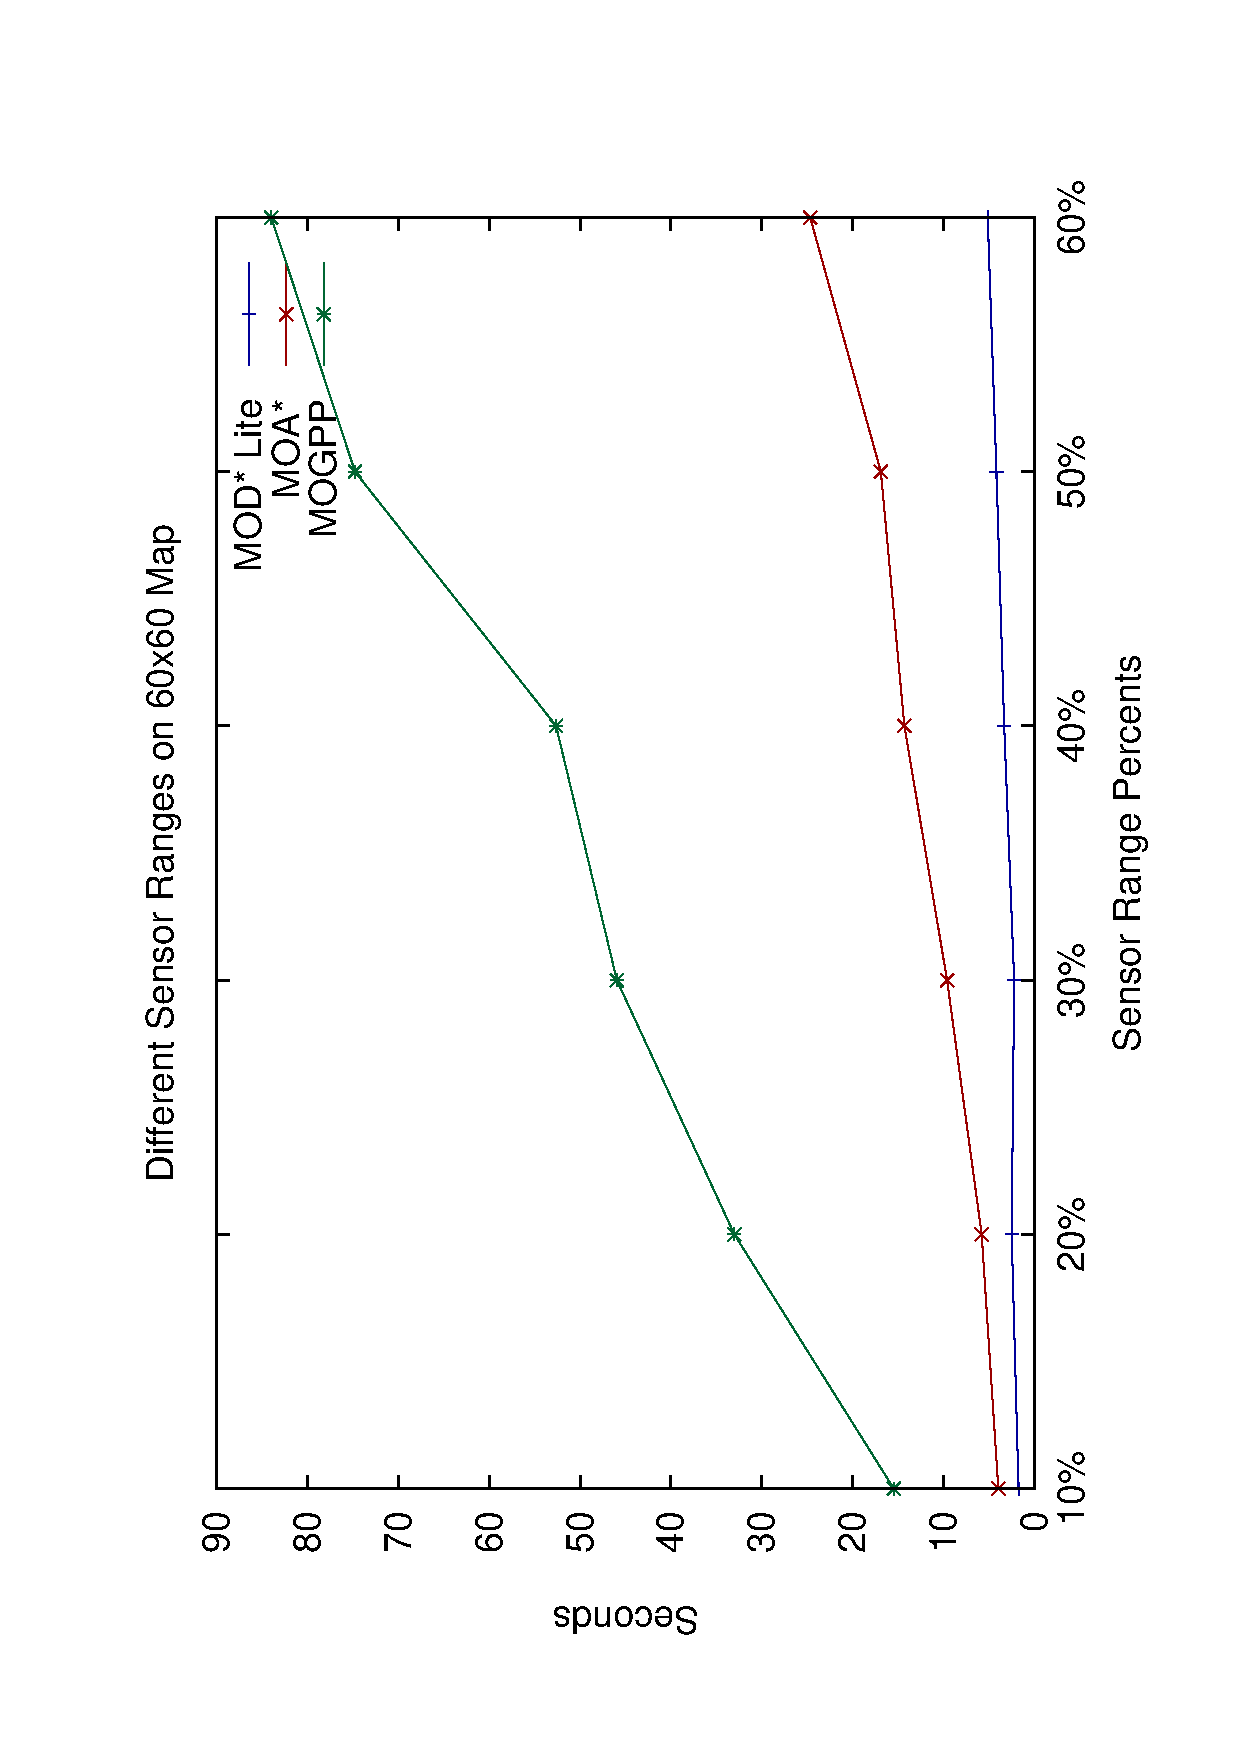
\includegraphics[width=2.5in, angle=270]{experimental/60x60_partially_normal}
\caption{60x60 Partially Observable Map on Different Sensor Ranges}
\label{fig:60x60sensor}
\end{figure}

\begin{figure}
\centering
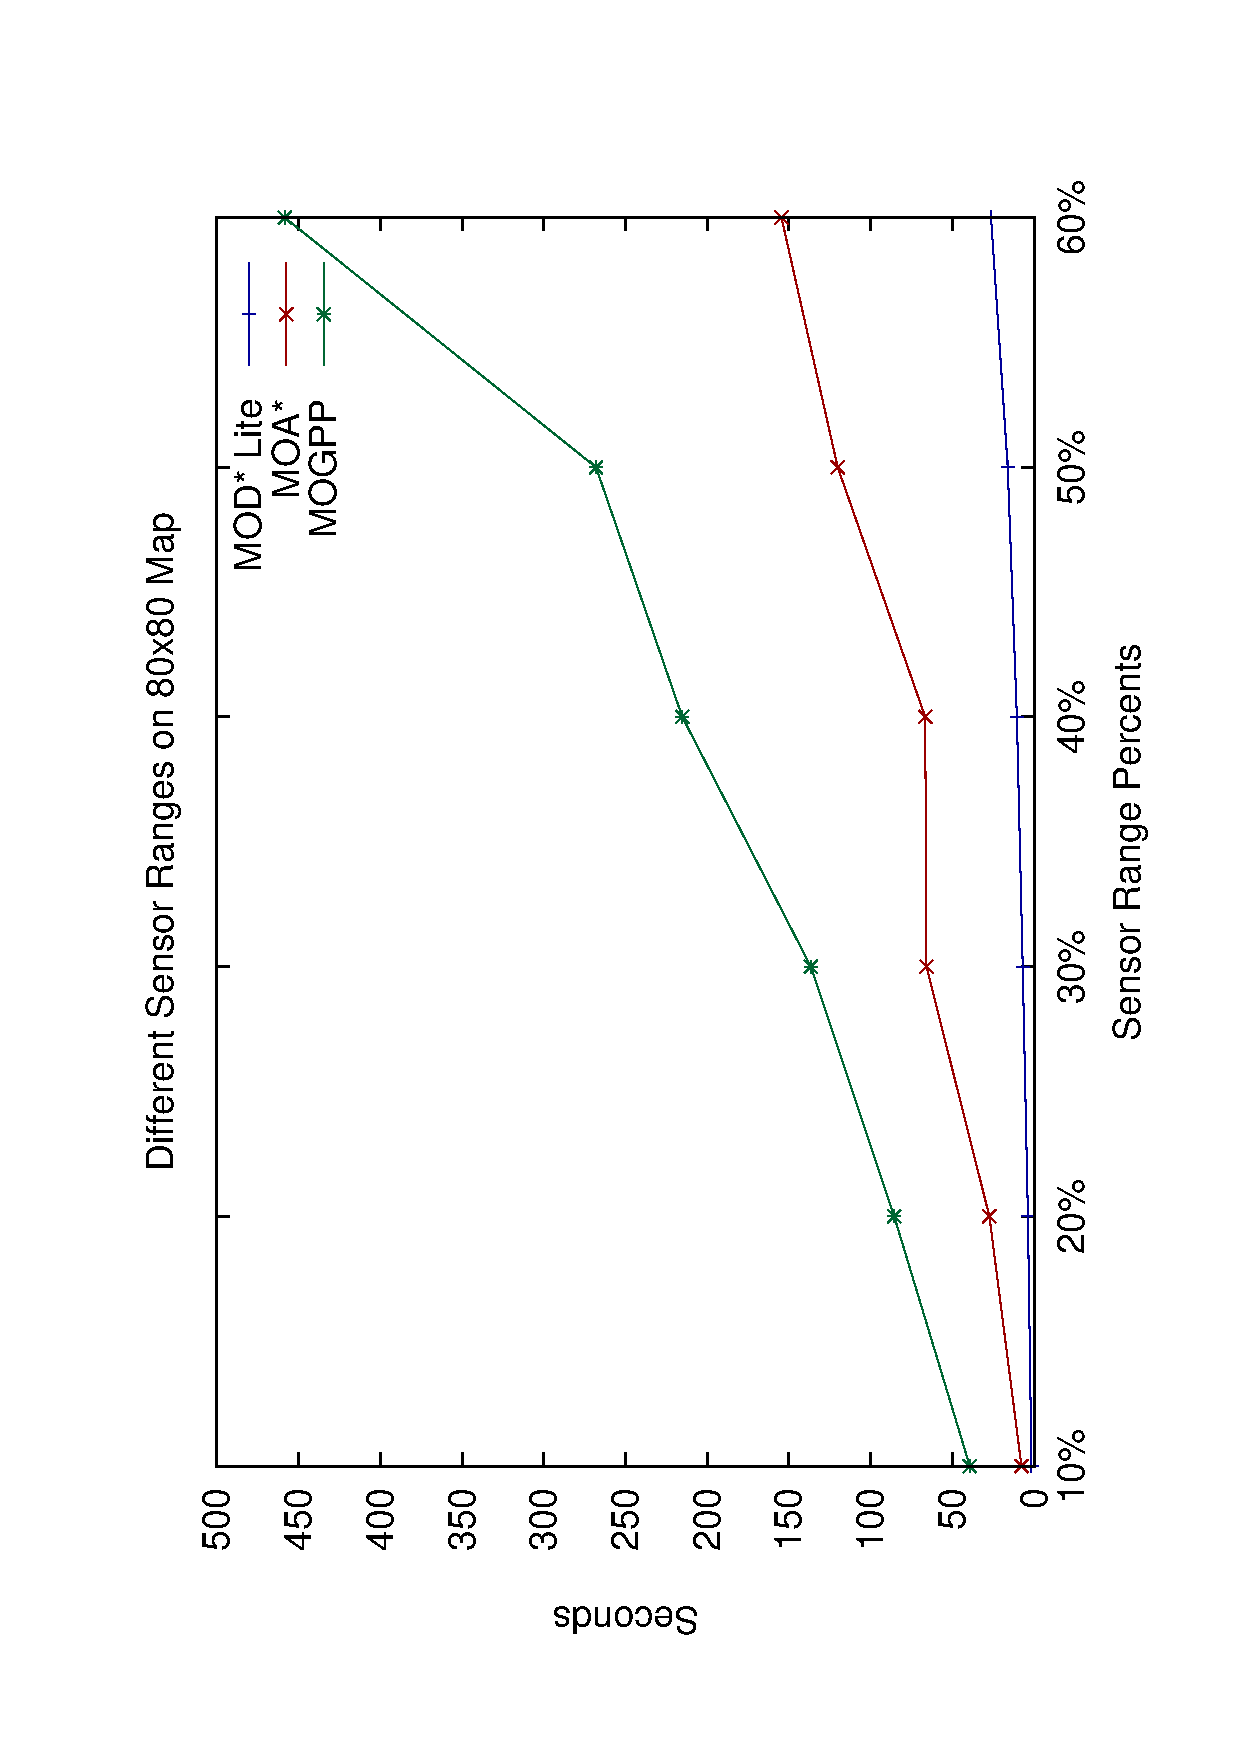
\includegraphics[width=2.5in, angle=270]{experimental/80x80_partially_normal}
\caption{80x80 Partially Observable Map on Different Sensor Ranges}
\label{fig:80x80sensor}
\end{figure}

\begin{figure}
\centering
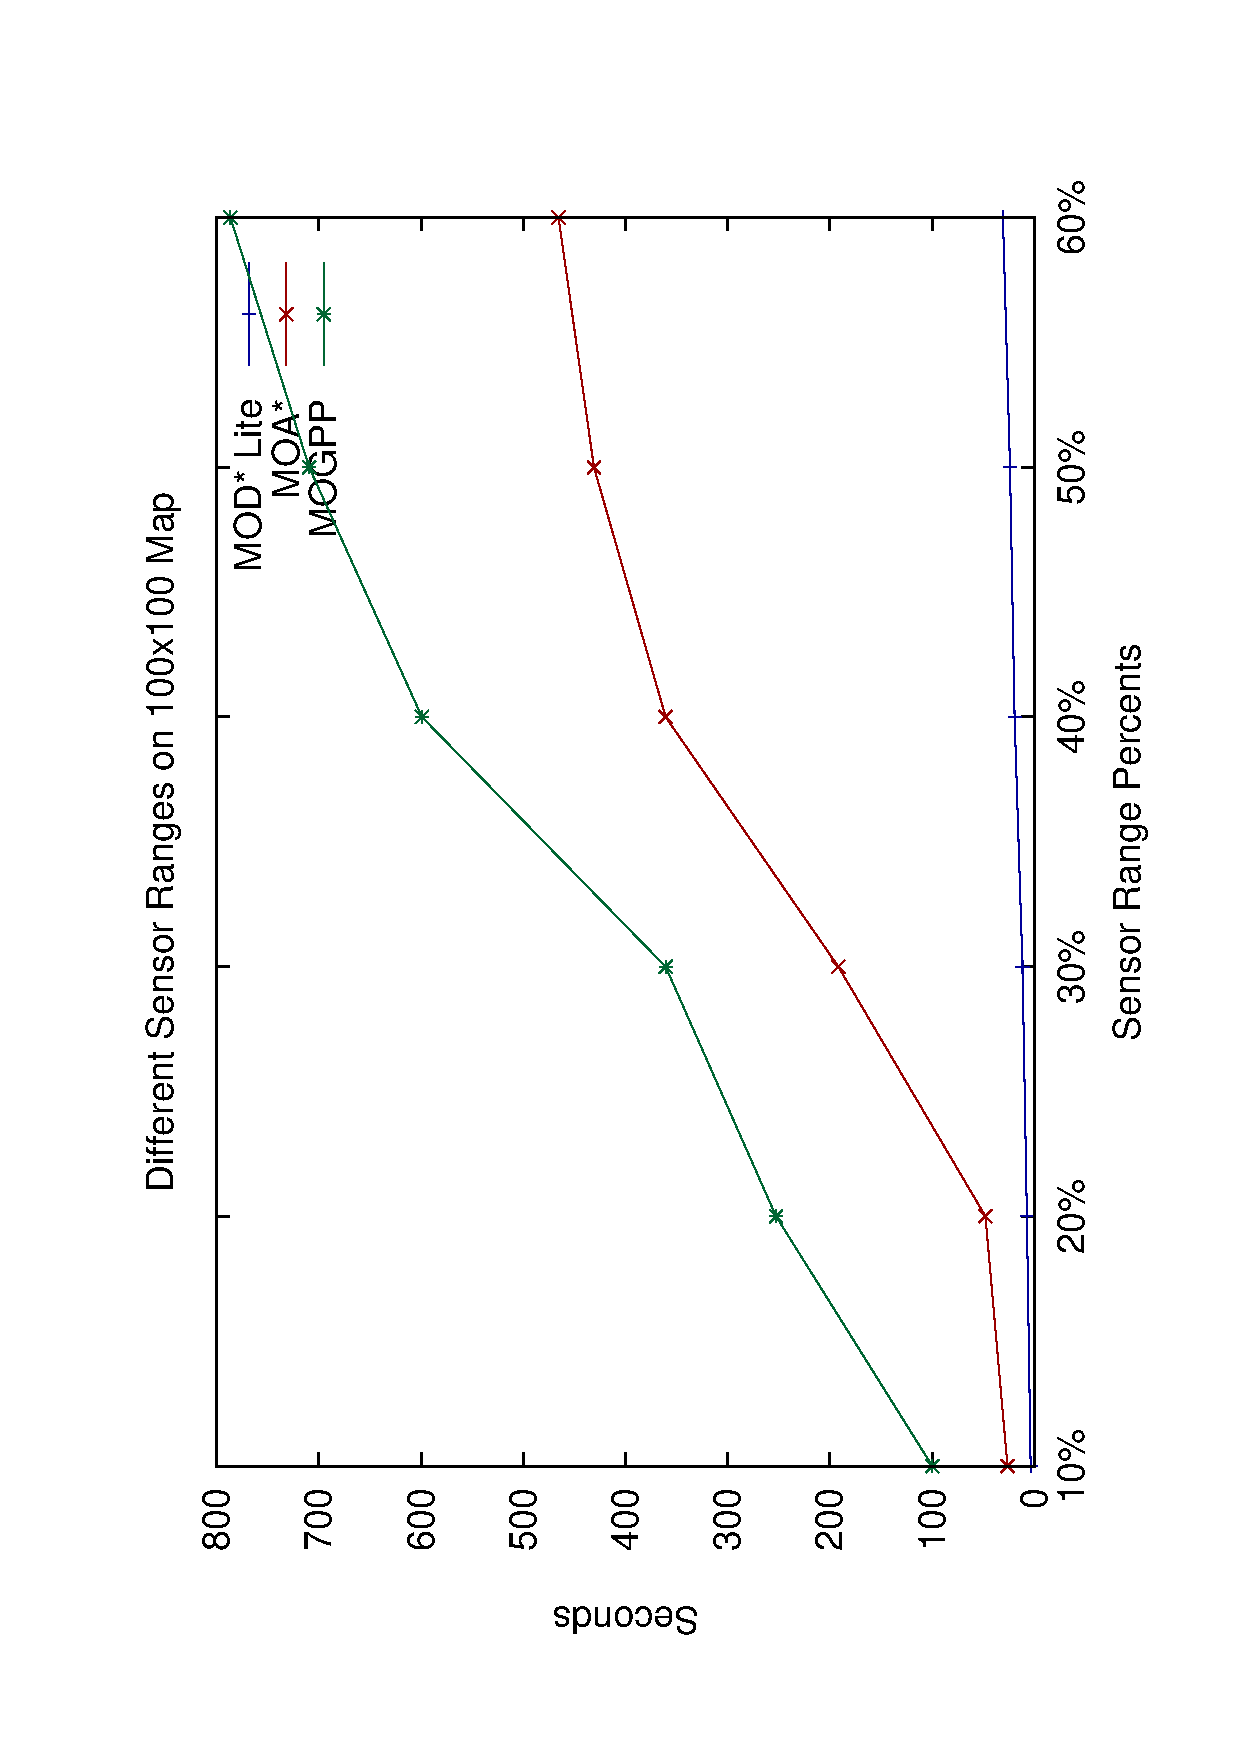
\includegraphics[width=2.5in, angle=270]{experimental/100x100_partially_normal}
\caption{100x100 Partially Observable Map on Different Sensor Ranges}
\label{fig:100x100sensor}
\end{figure}

\begin{figure}
\centering
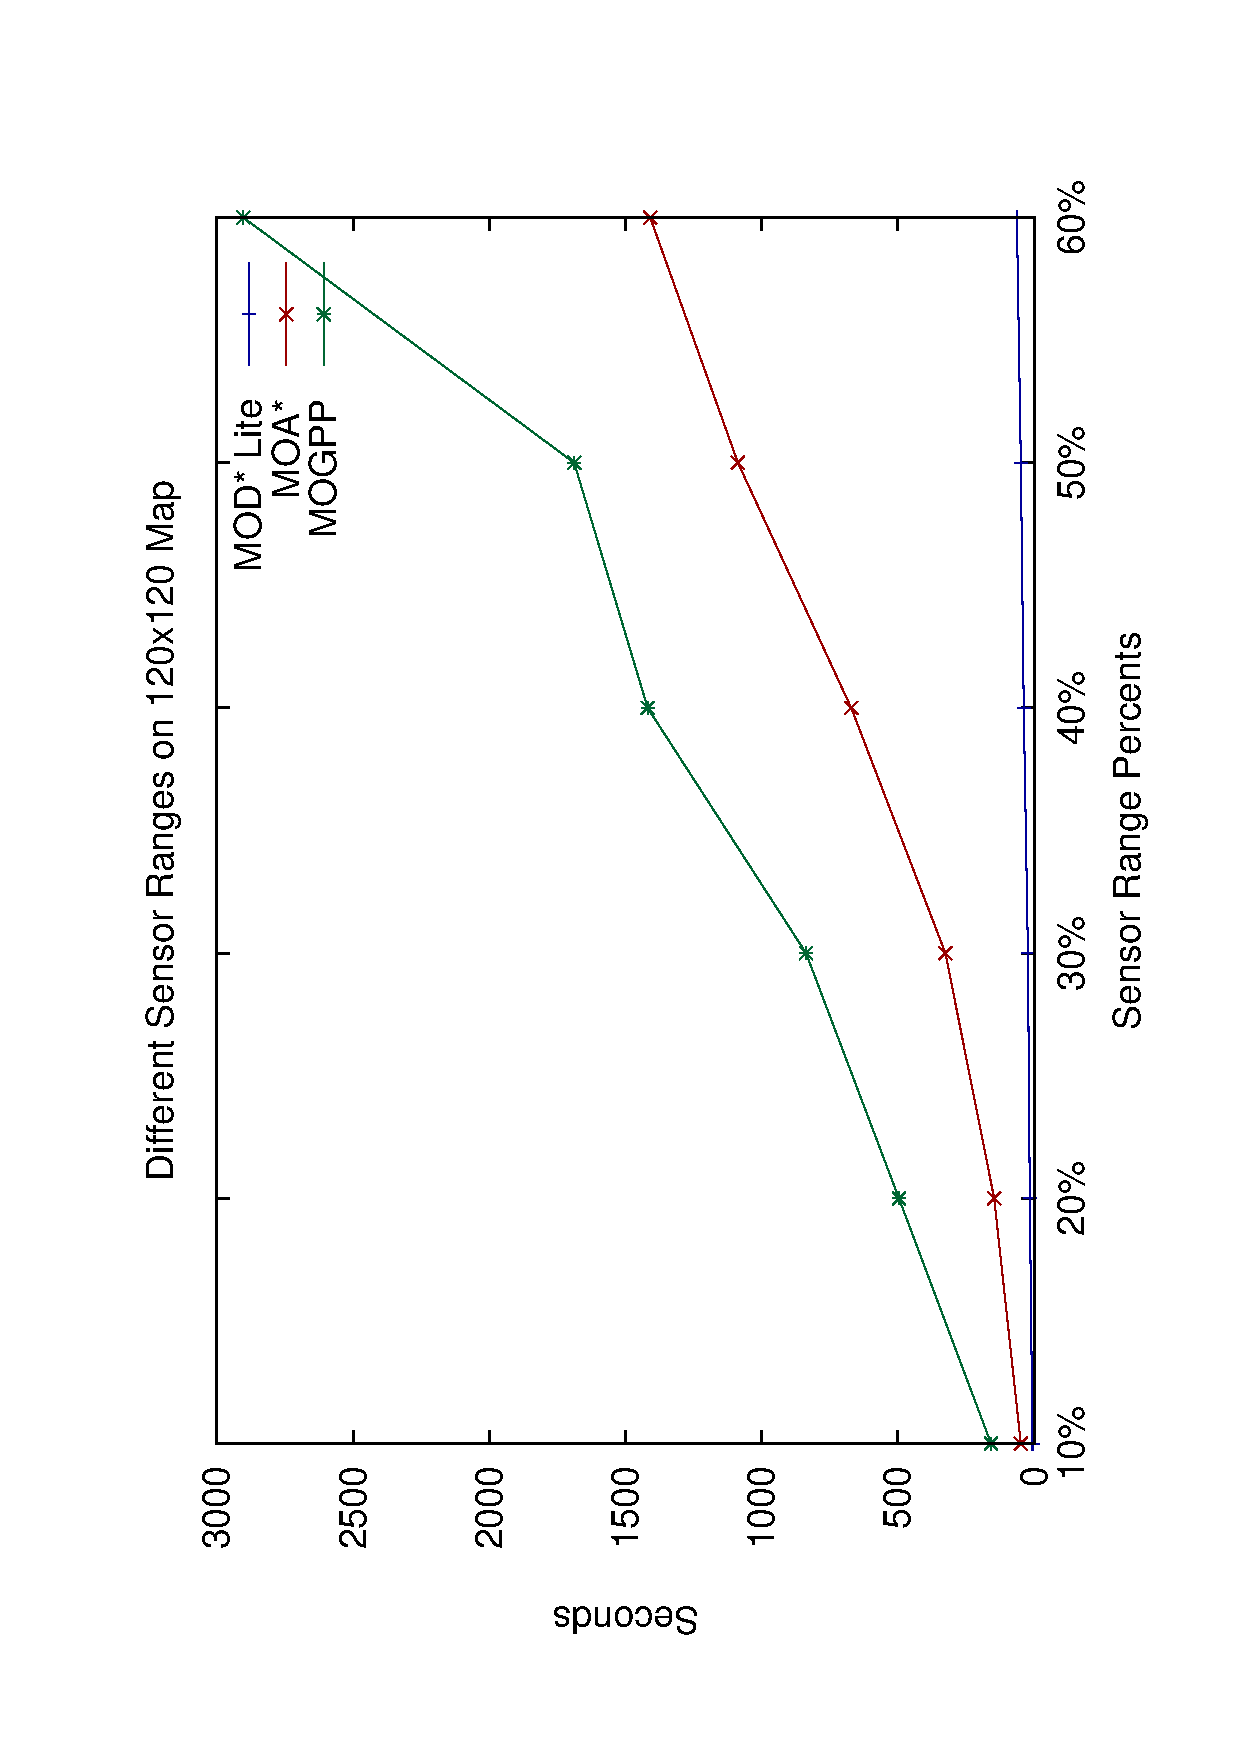
\includegraphics[width=2.5in, angle=270]{experimental/120x120_partially_normal}
\caption{120x120 Partially Observable Map on Different Sensor Ranges}
\label{fig:120x120sensor}
\end{figure}

\begin{figure}
\centering
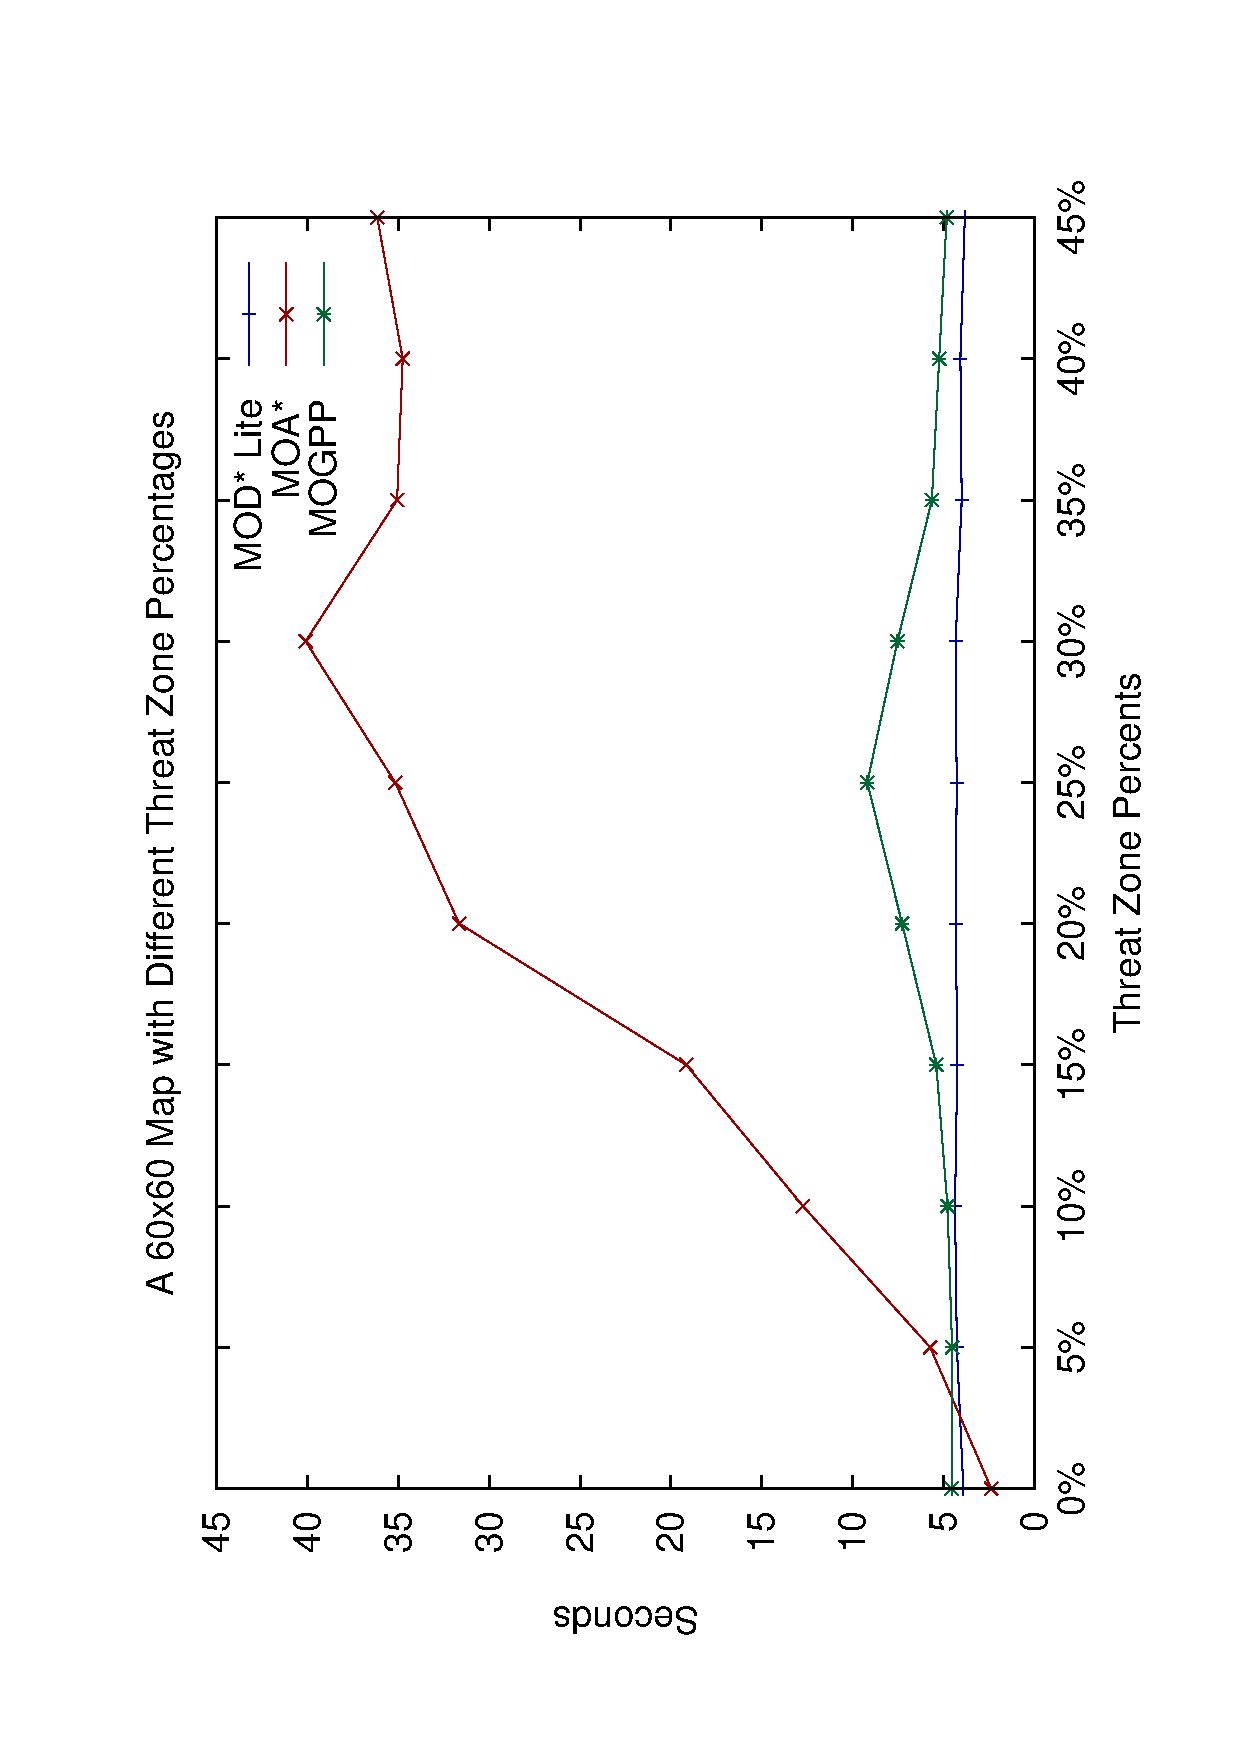
\includegraphics[width=2.5in, angle=270]{experimental/60x60_multiobj_normal}
\caption{Execution times of 60x60 Fully Observable Map on Different Threat Zone Percents}
\label{fig:tzratio60}
\end{figure}

\begin{figure}
\centering
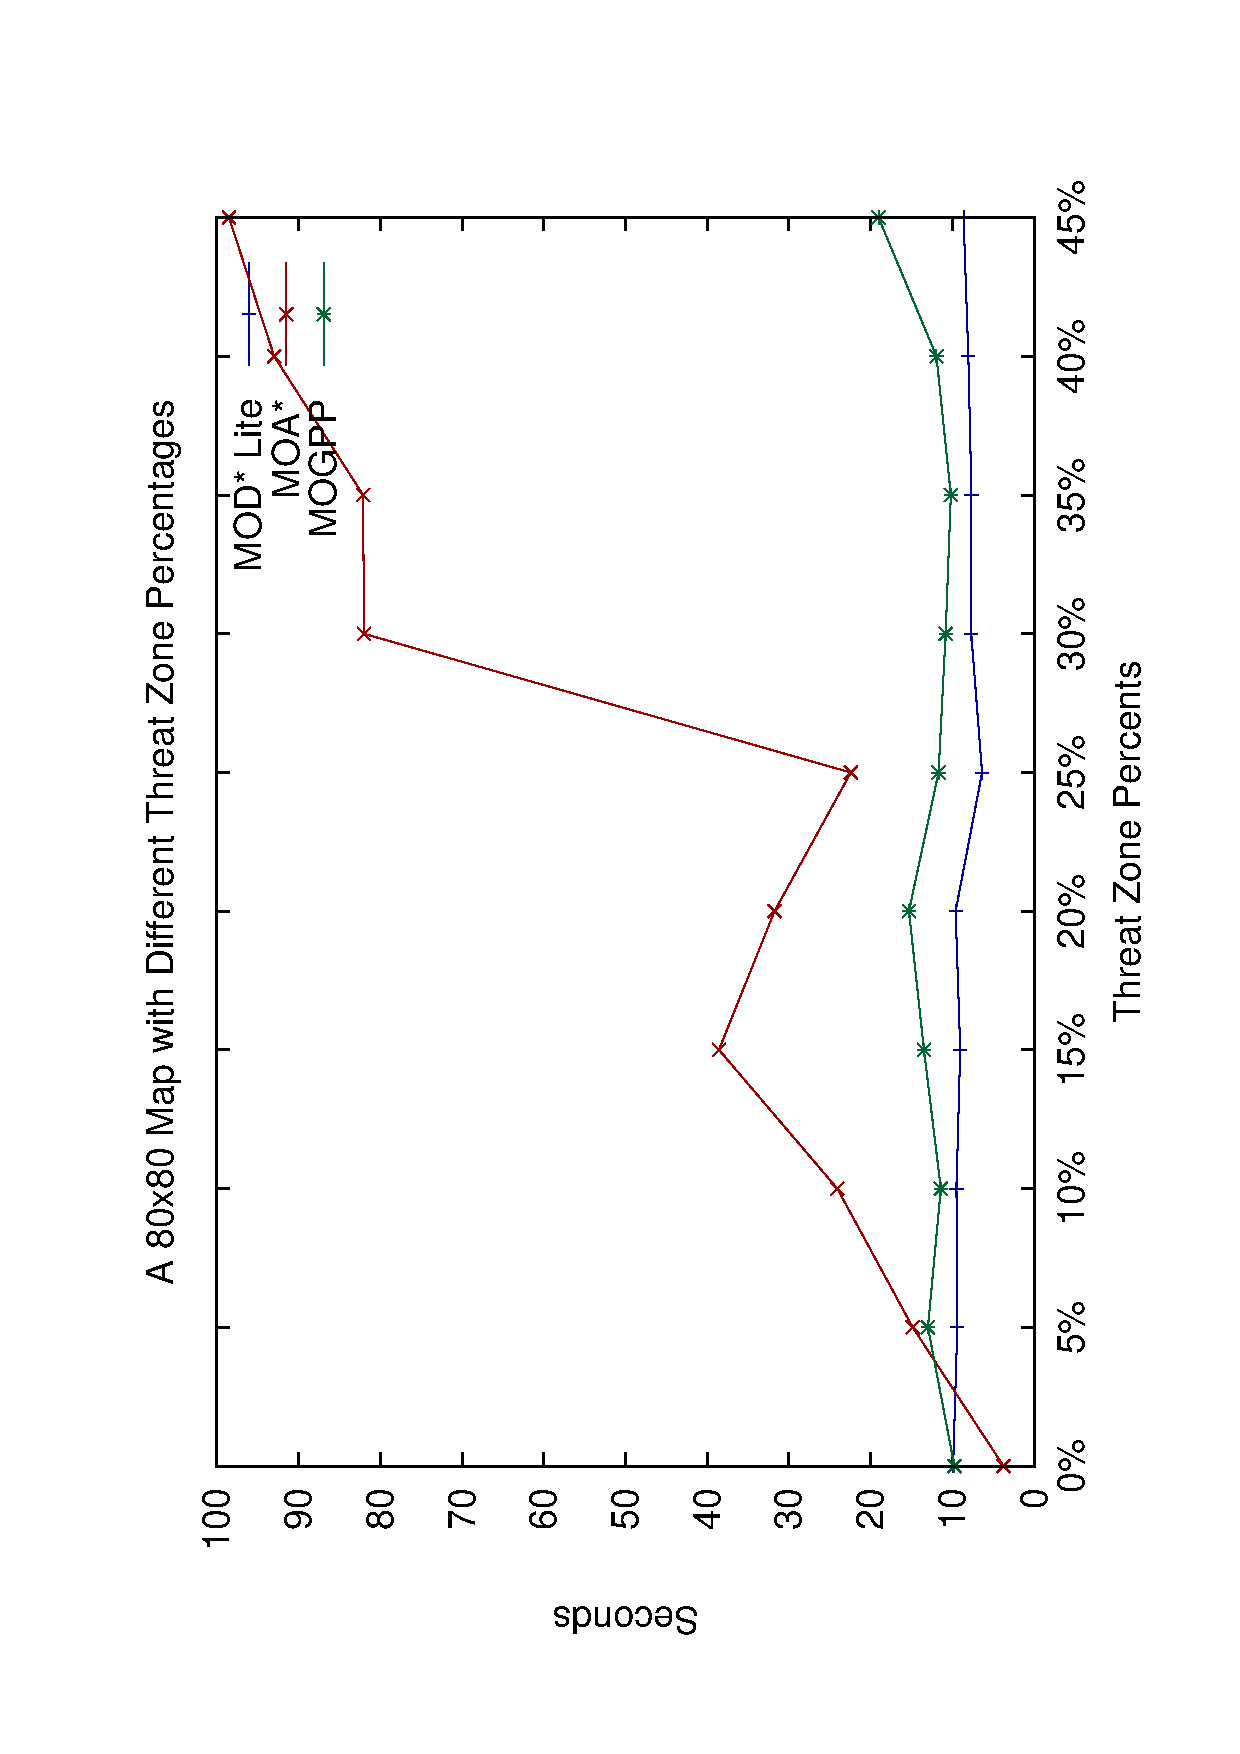
\includegraphics[width=2.5in, angle=270]{experimental/80x80_multiobj_normal}
\caption{Execution times of 80x80 Fully Observable Map on Different Threat Zone Percents}
\label{fig:tzratio80}
\end{figure}

%\begin{table}[ht]
%	\caption{MOGPP Execution Times on a 125x125 Partially Observable Map}
%	\centering
%    \begin{tabular}{l l}
%        \hline
%        Sensor Range	&	Execution Time (sec.)\\ [0.5ex] \hline
%        20\%			&	402.325\\
%        30\%			&	420.481\\
%		40\%			&	1024.237\\
%		50\%			&	1351.854\\
%		60\%			&	1922.415\\ [1ex]
%        \hline
%    \end{tabular}
%	\label{table:mogpp125vFrustum}
%\end{table}

The fundamental advantage of MOD* Lite can be seen very clearly on these tests. While MOD* Lite has the capability of updating only the effected states due to its incremental nature, MOA* re-plans the overall path from scratch when new parts become known and the weights of some cells have changed. This situation causes MOA* and MOGPP to work on exponentially long times. Total execution times to reach to the target for these test cases are given in Figures \ref{fig:60x60sensor}, \ref{fig:80x80sensor}, \ref{fig:100x100sensor} and \ref{fig:120x120sensor}. As can be seen from results, MOD* Lite can easily handle the dynamical issues of the environment where MOA* and MOGPP fails. Due to discovering different parts of the environment during execution, actual traversed path's costs of MOD* Lite, MOA* and MOGPP might be slightly different from each other, where MOD* Lite could follow a better path with respect to MOA* or MOGPP or vice versa.

\subsection{Multi Objectivity Tests}

As threat zones and their risk values are used as the second objective, percentages of these zones also effect execution time and generated path quality. In this set of tests different threat zone percents are tested on a fully observable 60 x 60 and 80 x 80 map and results are given in Figure \ref{fig:tzratio60} and \ref{fig:tzratio80}, respectively. It could be observed that increasing one of the objective' s ratio, or risks of threat zones for this test, does not effect performance of  MOD* Lite and MOGPP too much, they find results in approximately similar times. However, MOA* is tightly coupled with it and execution time increases gradually as the threat percentage increases.

\section{Conclusion and Future Work}
\label{chapter:conclusion}

Searching, path planning and navigation in virtual environments are vital issues and referred by many visualized real-world applications. These are recent problems and are considered in areas including robotics, virtual simulations or computer games and has been studied for many years. Computer science came up with many solutions considering on single criteria; i.e. shortest path from an initial location to a target location or safest path between two transition points. However, more complex situations where considering multiple objectives instead of a single objective for searching and finding an optimal or sub-optimal solution become more appropriate when it is desired to apply searching and navigation techniques to real world applications. On the other hand, one should not ignore interactive behaviour and dynamics of the real world and consider them for more realistic modelling. In a nutshell, a multi objective search algorithm which can work on partially observable dynamic environments is required to satisfy all of these requirements.

With this motivation; a novel approach for searching, planning and finding paths on known and unknown partially observable dynamic environments  where the agent needs to optimize more than one criteria that cannot be transformed to each other, MOD* Lite, is presented in this paper. MOD* Lite is based on D* Lite and it brings multi objectivity to the solution space successfully, which is required in many real-world problems. It is a domain independent algorithm and could be applied to any partially/fully observable dynamic virtual environment with $n$ different non-interacting objectives. It is compared with known and complete multi objective off-line path planning algorithm, MOA*, and also with a novel evolutionary solution, multi objective genetic path planner, MOGPP, based on solution quality and execution times. Experimental results show that MOD* Lite is able to optimize path quality and is fast enough to be used in real-world multi objective application areas such as robotics, computer games, and virtual simulations. According to the conducted literature survey and knowledge gained, MOD* Lite is the only and the one incremental search and navigation algorithm which could handle multi-objectivity.

There is an obvious gap on moving target multi objective path planning area. As there exists several incremental moving target solutions for virtual environment proposed within recent years \cite{Sun:2009}, \cite{GFR-A*Sun:2010}, \cite{MT-D*Lite:2010}; a modified versions of these solutions can be used with multi objectivity. Also MOD* Lite could be reconsidered in multi agent perspective where each agent distributively execute their planners and cooperate to reach a target location. Thus, further studies will include incremental moving target multi objective problems, their solutions and multi-agent perspective.

\bibliography{journal}{}
\bibliographystyle{ieeetr}

\end{document}
